\chapter{Evaluation}
\label{sec:evaluation}

In the evaluation phase of the work we compare our parser plugins. For that purpose we first describe our comparison criteria in the first section of this chapter. After that we measure and analyze the plugins according to each criteria in the following sections. At the end we determine the plugins that best fit our criteria.

\section{Goals}

The goal of this evaluation is to find one or more parser plugin that
\begin{itemize}
  \item are fast,
  \item have low resource usage,
  \item use code that is
    \begin{itemize}
      \item both maintainable and
      \item easily extendible, and
    \end{itemize}
  \item has good error reporting capabilities.
\end{itemize}

To make sure that the plugins are reasonably fast we compare their execution time using runtime benchmarks and answer~\Cref{que:speed}.

  \speed*

For the resource usage we analyze the heap memory consumption. To make sure that the plugins are maintainable we analyze code sizes and take a look at the \glsdesc{CC}. We also examine the extensibility and composability of the plugins looking at code changes for specific bug fixes and feature additions. This step will help us to answer~\Cref{que:closeness}.

  \closeness*

To make sure the plugins produce good error messages we also compare these messages for specific input files in a detailed analysis.

\section{Performance Analysis}

In the following section we analyze the runtime time and memory usage of our plugins for certain input files. We first describe the overall methodical steps we took for both the runtime and memory benchmarks. Then we describe, measure and analyze both of these criteria in their own sections.

\subsection{Method}

To make all benchmarks reproducible we start by detailing the whole setup including used hardware, software, build configuration options and how we generated the input files.

\subsubsection{Hardware}

For all of the tests we used the hardware described in Table~\ref{table:benchmark_hardware}.

\begin{table}[H]
  \caption{Hardware Setup}
  \label{table:benchmark_hardware}
  \centering
  \begin{tabular}{ll}
\toprule
\multicolumn{2}{c}{MacBook Pro (Retina, 15-inch, Late 2013)}\\
\midrule
               CPU &            i7-4960HQ\\
                   &              2.6 GHz\\
                   &        6 MB L3 Cache\\
                   &      128 MB L4 Cache\\
               RAM &                16 GB\\
                   &        1600 MHz DDR3\\
                HD &    Apple SSD SM1024F\\
                   &                 1 TB\\
\bottomrule
  \end{tabular}
\end{table}

\subsubsection{Software}

Table~\ref{table:benchmark_software} shows the overall software setup for the benchmarks. We tested the performance both on macOS and Linux. For the Linux setup we used the Mac version of Docker. The basis of the runtime benchmark is \href{https://github.com/ElektraInitiative/libelektra/commit/54a4c0194946917b7d093e0777f465619b2f3d6f}{commit 54a4c019} of Elektra’s code base, while we measured the memory usage using \href{https://github.com/ElektraInitiative/libelektra/commit/ea418f177a5e2707f59f61b5e130a596abdd1c56}{commit ea418f17}. No code of any of the tested plugins changed \href{https://github.com/ElektraInitiative/libelektra/compare/54a4c0194946917b7d093e0777f465619b2f3d6f...ea418f177a5e2707f59f61b5e130a596abdd1c56}{between those two commits}.

\begin{table}[H]
    \newcommand{\YAEP}{{\href{https://github.com/vnmakarov/yaep/commit/550de4cc5600d5f6109c7ebcfbacec51bf80d8d3}{YAEP 550de4cc}}}
    \caption{Software Setup}
    \label{table:benchmark_software}
    \begin{subtable}[t]{.45\linewidth}
      \centering
        \caption{Mac Setup}
        \label{table:benchmark_mac}
        \begin{tabular}{ll}
\toprule
                OS &        macOS 10.14.5\\
                   &                     \\
\midrule
          Compiler &          Clang 8.0.0\\
        Generators &          ANTLR 4.7.2\\
                   &          Bison 3.4.1\\
         Libraries &       yaml-cpp 0.6.2\\
                   &                \YAEP\\
                   &          PEGTL 2.8.0\\
    Other Software &         CMake 3.14.4\\
                   &          Ninja 1.9.0\\
                   &      hyperfine 1.5.0\\
                   &            cloc 1.82\\
\bottomrule
        \end{tabular}
    \end{subtable}
    \begin{subtable}[t]{.45\linewidth}
      \centering
        \caption{Linux Setup}
        \label{table:benchmark_docker}
        \begin{tabular}{ll}
\toprule
            Docker &    18.09.2, build 6247962\\
        Base Image & Debian sid (sid-20190506)\\
\midrule
         Compilers &     Clang 6.0.1/GCC 8.3.0\\
        Generators &               ANTLR 4.7.2\\
                   &               Bison 3.3.2\\
         Libraries &            yaml-cpp 0.6.2\\
                   &                     \YAEP\\
                   &               PEGTL 2.7.1\\
    Other Software &              CMake 3.13.4\\
                   &               Ninja 1.8.2\\
                   &           hyperfine 1.5.0\\
\bottomrule
        \end{tabular}
    \end{subtable}
\end{table}

\subsubsection{Build Setup}

The following list shows the \href{https://cmake.org}{CMake} options that we used for all benchmarks:

\begin{itemize}
  \item \sh{-GNinja},
  \item \sh{-DPLUGINS=ALL},
  \item \sh{-DCMAKE_BUILD_TYPE=Release},
  \item \sh{-DENABLE_LOGGER=OFF}, and
  \item \sh{-DENABLE_DEBUG=OFF}.
\end{itemize}

\subsubsection{Input}

\newcommand{\URLKeyFramesJSON}{https://master.libelektra.org/src/plugins/yajl/yajl/keyframes_complex.json}

\newcommand{\FileKeyFrames}{{%
\codebox{%
\href{http://rawdata.libelektra.org/tree/master/YAML/Input/keyframes.yaml}%
{\textcolor{black}{\texttt{keyframes.yaml}}}}%
}}
\newcommand{\FileCombined}{{%
\codebox{%
\href{http://rawdata.libelektra.org/tree/master/YAML/Input/combined.yaml}%
{\textcolor{black}{\texttt{combined.yaml}}}}%
}}
\newcommand{\FileGenerated}{{%
\codebox{%
\href{http://rawdata.libelektra.org/tree/master/YAML/Input/generated.yaml}%
{\textcolor{black}{\texttt{generated.yaml}}}}%
}}
\newcommand{\FileGeneratedHundredThousand}{{%
\codebox{%
\href{http://rawdata.libelektra.org/tree/master/YAML/Input/generated_100000.yaml}%
{\textcolor{black}{\texttt{generated\_100000.yaml}}}}%
}}
\newcommand{\FileGenerateYAML}{{%
\codebox{%
\href{https://master.libelektra.org/scripts/generate-yaml}%
{\textcolor{black}{\texttt{generate-yaml}}}}%
}}
\newcommand{\FileCutInput}{{%
\codebox{%
\href{http://rawdata.libelektra.org/tree/master/YAML/Scripts/cut_input}%
{\textcolor{black}{\texttt{cut\_input}}}}%
}}

As first input for the benchmarks we used a \href{\URLKeyFramesJSON}{JSON configuration file} of the \href{https://www.libelektra.org/plugins/yajl}{YAJL plugin} that we converted to block syntax using the \LinkYAMLCPP{} plugin. We then modified the exported data by removing all \yaml{!<!elektra/meta>} tags, which are not supported by the other \glstext{YAML} plugins. We call the resulting file \FileKeyFrames{} in the remainder of the thesis. This file and all other data of the benchmark is available here:

\begin{leftbar}
  \url{http://rawdata.libelektra.org/tree/master/YAML}
\end{leftbar}

. For another input file called \FileCombined{} we copy and pasted parts of test data and various other \glstext{YAML} files in Elektra’s repository into a single file. While the file content is nonsensical, it should at least contains a mix of \glstext{YAML} data that covers most of the code paths of the \glstext{YAML} plugins.

Since both of these files are relatively small, \FileKeyFrames{} contains 218 lines, while \FileCombined{} contains 152 lines, we also generated data using a Python script that we called \FileGenerateYAML{}. This script generates \glstext{YAML} maps using \href{https://en.wikipedia.org/wiki/Universally_unique_identifier}{\glspl{UUID}} as scalar keys and values. For the \glstext{YAML} scalars the script randomly selects one of the three flow scalar styles:

\begin{itemize}
  \item single quoted scalar,
  \item double quoted scalar, or
  \item plain scalar
\end{itemize}

. This always works since \glspl{UUID} contain no character sequence that has special meaning according to the \glstext{YAML} specification. Using this method we generated two files:

\begin{itemize}
  \item \FileGenerated{} that contains 10 000 lines, and

  \item \FileGeneratedHundredThousand{} that contains 100 000 lines
\end{itemize}

. We also created another script called \FileCutInput{} to generate additional smaller input files that contain the first 50000, 10000, 5000, 1000, 500, 100, 50, 10, 5 and 1 lines of \FileGeneratedHundredThousand{}.

\subsection{Runtime Performance}
\label{sec:run_time_performance}

\subsubsection{Method}

\newcommand{\FilePluginGetSet}{{%
\codebox{%
\href{https://master.libelektra.org/benchmarks/plugingetset.c}%
{\textcolor{black}{\texttt{benchmark\_plugingetset}}}}%
}}
\newcommand{\FileBenchmarkYAML}{{%
\codebox{%
\href{https://master.libelektra.org/scripts/benchmark-yaml.in}%
{\textcolor{black}{\texttt{benchmark-yaml}}}}%
}}
\newcommand{\FileBenchmarkRuntime}{{%
\codebox{%
\href{http://rawdata.libelektra.org/tree/master/YAML/Scripts/benchmark-runtime}%
{\textcolor{black}{\texttt{benchmark-runtime}}}}%
}}
\newcommand{\ToolHyperfine}{{%
\codebox{%
\href{https://github.com/sharkdp/hyperfine}%
{\textcolor{black}{\texttt{hyperfine}}}}%
}}

To compare the runtime performance we used the C application \FilePluginGetSet{} that opens an Elektra plugin using a specific configuration file. For the whole benchmark process we created a Bash script, called \FileBenchmarkYAML{}, that uses the benchmarking tool \ToolHyperfine{} to call \FilePluginGetSet{} using different \glstext{YAML} plugins. Figure~\ref{fig:benchmark} shows a diagram of this setup.

\begin{figure}[H]
  \centering
    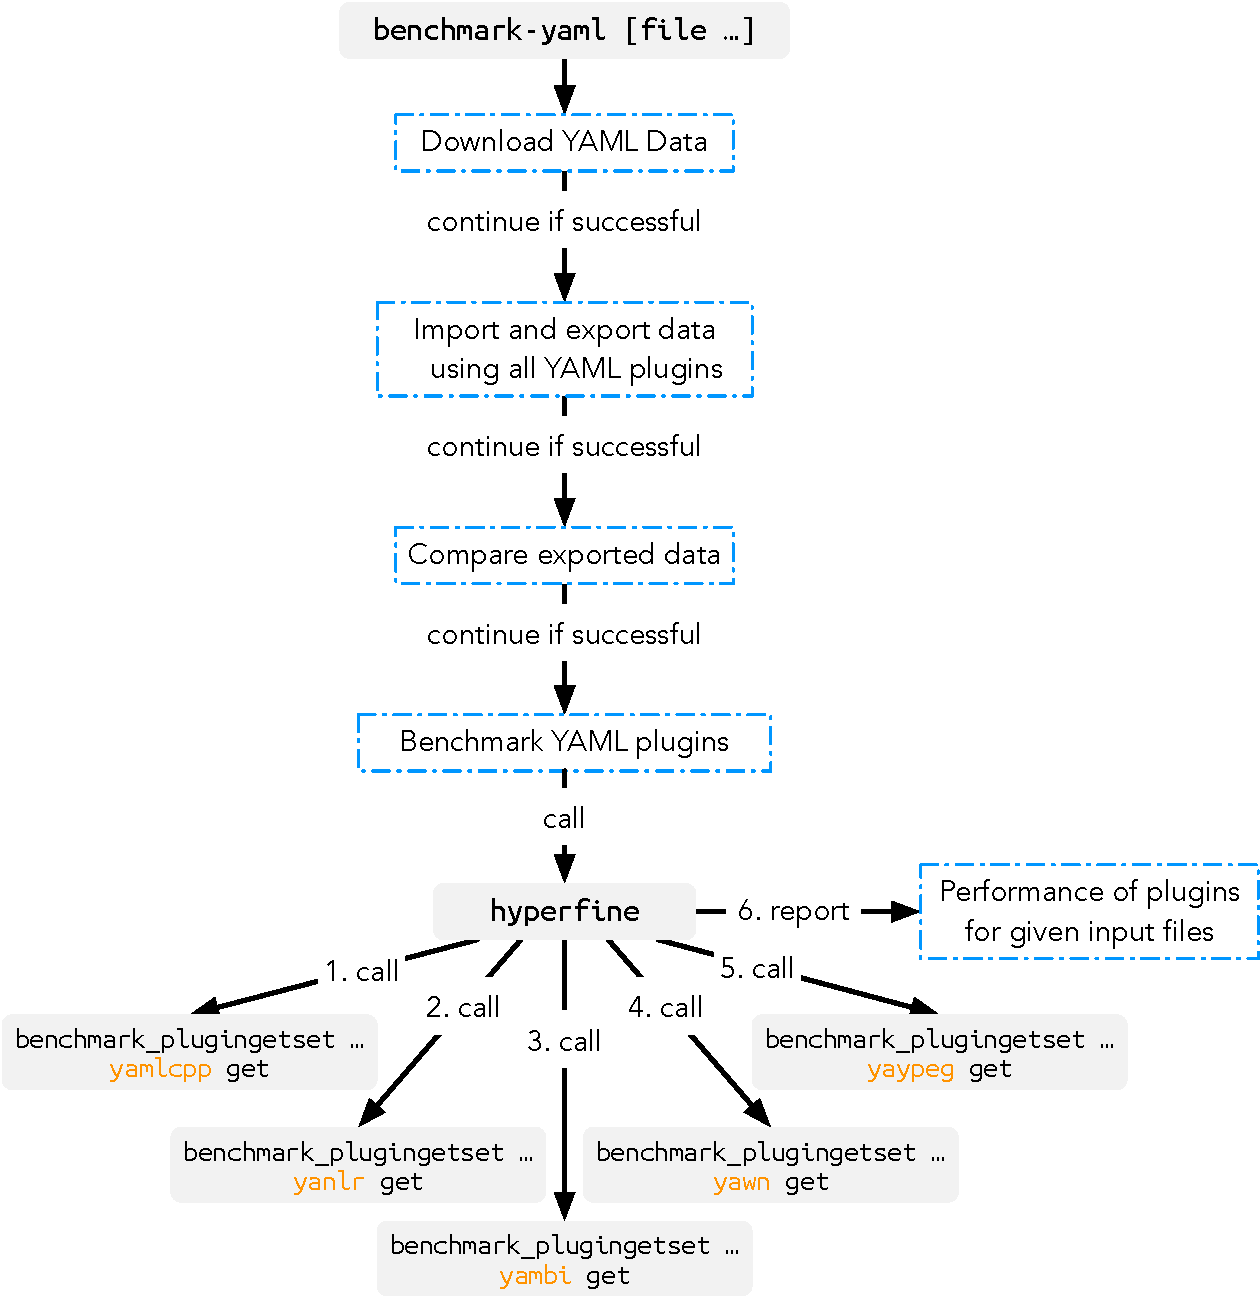
\includegraphics[width=0.9\textwidth]{Benchmark}
  \caption{The diagram above shows the basic sequence of steps to measure the runtime performance of the \glstext{YAML} plugins.}
  \label{fig:benchmark}
\end{figure}

For the measurement we use \ToolHyperfine{}, since this tool

\begin{enumerate}
  \item automatically determines how often it should call \FilePluginGetSet{} for meaningful measurement results,
  \item shows us when it is time to redo the benchmark, by informing us about statistical outliers, and
  \item prints important statistical data such as the mean runtime and the standard derivation.
\end{enumerate}

To make sure we repeat the benchmark every time \href{https://github.com/sharkdp/hyperfine}{\sh{hyperfine}} reports statistical outliers we created the Shell script \FileBenchmarkRuntime{}. This script calls \FileBenchmarkYAML{} for every input file and repeats a benchmark, until \href{https://github.com/sharkdp/hyperfine}{\sh{hyperfine}} does not report any warnings. The script \FileBenchmarkRuntime{} \emph{does} ignore warnings about runtimes under 5 milliseconds though, since \FilePluginGetSet{} might take less execution time for small \glstext{YAML} files.

\subsubsection{Results}

The graphs in this section show the results of the benchmark for different input files.

\begin{figure}[H]
  \begin{bchart}[max=30, width=0.8\textwidth, unit=ms]
    \bcbar[text=17.7 ± 0.7, value=macOS, color=orange]{17.7}
    \bcbar[text=25.5 ± 3.5, value=Linux/GCC, color=orange]{25.5}
    \bcbar[text=24.2 ± 2.9, value=Linux/Clang, color=orange]{24.2}

    \bcbar[text=15.8 ± 0.8, value=macOS, color=DarkYellow]{15.8}
    \bcbar[text=27.3 ± 2.3, value=Linux/GCC, color=DarkYellow]{27.3}
    \bcbar[text=25.8 ± 1.6, value=Linux/Clang, color=DarkYellow]{25.8}

    \bcbar[text=18.7 ± 1, value=macOS, color=Turquoise3]{18.7}
    \bcbar[text=20.1 ± 1.8, value=Linux/GCC, color=Turquoise3]{20.1}
    \bcbar[text=20.1 ± 1.6, value=Linux/Clang, color=Turquoise3]{20.1}

    \bcbar[text=13.8 ± 0.7, value=macOS, color=Aqua]{15.4}
    \bcbar[text=21.6 ± 1.8, value=Linux/GCC, color=Aqua]{21.6}
    \bcbar[text=19.8 ± 1.1, value=Linux/Clang, color=Aqua]{19.8}

    \bcbar[text=23.8 ± 1, value=macOS, color=DarkOrchid]{23.8}
    \bcbar[text=22.8 ± 2.2, value=Linux/GCC, color=DarkOrchid]{22.8}
    \bcbar[text=22.3 ± 2.1, value=Linux/Clang, color=DarkOrchid]{22.3}
  \end{bchart}
  \begin{center}
  \vspace{-0.5cm}
    \tikzcircle{orange} YAML CPP ~~
    \tikzcircle{DarkYellow} Yan LR ~~
    \tikzcircle{Turquoise3} YAMBi ~~
    \tikzcircle{Aqua} YAwn ~~
    \tikzcircle{DarkOrchid} YAy PEG
  \vspace{-0.5cm}
  \end{center}
  \caption{This bar chart shows the run time of the plugins for the input \FileKeyFrames{}.}
  \label{fig:benchmark_keyframes}
\end{figure}

\begin{figure}[H]
  \begin{bchart}[max=30, width=0.8\textwidth, unit=ms]
    \bcbar[text=12.3 ± 0.9, value=macOS, color=orange]{12.3}
    \bcbar[text=24.1 ± 2.7, value=Linux/GCC, color=orange]{24.1}
    \bcbar[text=22.2 ± 2.5, value=Linux/Clang, color=orange]{22.2}

    \bcbar[text=9.3 ± 0.5, value=macOS, color=DarkYellow]{9.3}
    \bcbar[text=24.6 ± 1.5, value=Linux/GCC, color=DarkYellow]{24.6}
    \bcbar[text=22.8 ± 1.5, value=Linux/Clang, color=DarkYellow]{22.8}

    \bcbar[text=11.9 ± 0.8, value=macOS, color=Turquoise3]{11.9}
    \bcbar[text=19.4 ± 1.4, value=Linux/GCC, color=Turquoise3]{19.4}
    \bcbar[text=18.9 ± 1.9, value=Linux/Clang, color=Turquoise3]{18.9}

    \bcbar[text=8.2 ± 0.6, value=macOS, color=Aqua]{8.2}
    \bcbar[text=20.2 ± 1.9, value=Linux/GCC, color=Aqua]{20.2}
    \bcbar[text=21.5 ± 4.2, value=Linux/Clang, color=Aqua]{21.5}

    \bcbar[text=14.3 ± 0.7, value=macOS, color=DarkOrchid]{14.3}
    \bcbar[text=20.3 ± 1.8, value=Linux/GCC, color=DarkOrchid]{20.3}
    \bcbar[text=19.7 ± 3.2, value=Linux/Clang, color=DarkOrchid]{19.7}
  \end{bchart}
  \begin{center}
  \vspace{-0.5cm}
    \tikzcircle{orange} YAML CPP ~~
    \tikzcircle{DarkYellow} Yan LR ~~
    \tikzcircle{Turquoise3} YAMBi ~~
    \tikzcircle{Aqua} YAwn ~~
    \tikzcircle{DarkOrchid} YAy PEG
  \vspace{-0.5cm}
  \end{center}
  \caption{This bar chart shows the run time of the plugins for the input \FileCombined{}.}
  \label{fig:benchmark_combined}
\end{figure}

\begin{figure}[H]
  \begin{bchart}[max=385, width=0.8\textwidth, unit=ms]
    \bcbar[text=239.5 ± 4.3, value=macOS, color=orange]{239.5}
    \bcbar[text=139.4 ± 2.8, value=Linux/GCC, color=orange]{139.4}
    \bcbar[text=137.3 ± 11.8, value=Linux/Clang, color=orange]{137.3}

    \bcbar[text=119.9 ± 1.1, value=macOS, color=DarkYellow]{119.9}
    \bcbar[text=123.7 ± 2.2, value=Linux/GCC, color=DarkYellow]{123.7}
    \bcbar[text=124.5 ± 5.2, value=Linux/Clang, color=DarkYellow]{124.5}

    \bcbar[text=174.8 ± 1.7, value=macOS, color=Turquoise3]{174.8}
    \bcbar[text=65 ± 2.4, value=Linux/GCC, color=Turquoise3]{65}
    \bcbar[text=64.8 ± 2.5, value=Linux/Clang, color=Turquoise3]{64.8}

    \bcbar[text=73.6 ± 1, value=macOS, color=Aqua]{73.6}
    \bcbar[text=77.3 ± 2.6, value=Linux/GCC, color=Aqua]{77.3}
    \bcbar[text=74.9 ± 3.1, value=Linux/Clang, color=Aqua]{74.9}

    \bcbar[text=363.2 ± 2, value=macOS, color=DarkOrchid]{363.2}
    \bcbar[text=156.8 ± 5.7, value=Linux/GCC, color=DarkOrchid]{156.8}
    \bcbar[text=161.1 ± 7.5, value=Linux/Clang, color=DarkOrchid]{161.1}
  \end{bchart}
  \begin{center}
  \vspace{-0.5cm}
    \tikzcircle{orange} YAML CPP ~~
    \tikzcircle{DarkYellow} Yan LR ~~
    \tikzcircle{Turquoise3} YAMBi ~~
    \tikzcircle{Aqua} YAwn ~~
    \tikzcircle{DarkOrchid} YAy PEG
  \vspace{-0.5cm}
  \end{center}
  \caption{This bar chart shows the run time of the plugins for the input \FileGenerated{}.}
  \label{fig:benchmark_generated}
\end{figure}

\begin{figure}[H]
  \centering
    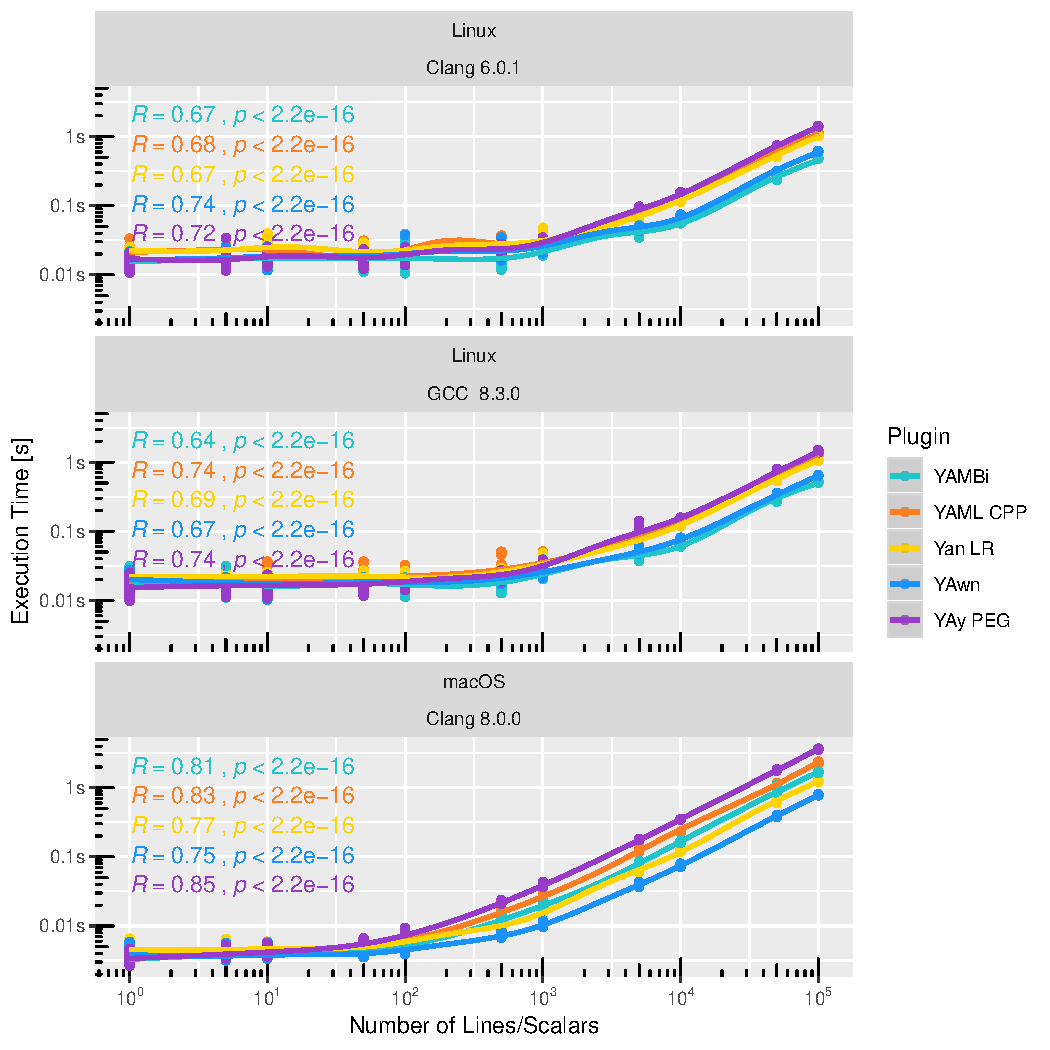
\includegraphics[width=\textwidth]{BenchmarkResultRuntime}
  \caption{The diagrams above show the runtime of the plugins for the input file \FileGeneratedHundredThousand{} and other files that contain only the first $n$ number of lines of this file.}
  \label{fig:benchmark_results_generated}
\end{figure}

\subsubsection{Analysis}

If we look at Figure~\ref{fig:benchmark_results_generated} we see that the runtime seems to grow linearly after a certain number of input lines. To verify this hypothesis we removed all samples with a line length smaller than 1000. Figure~\ref{fig:benchmark_results_generated_above_1000} shows the result.

\begin{figure}[H]
  \centering
    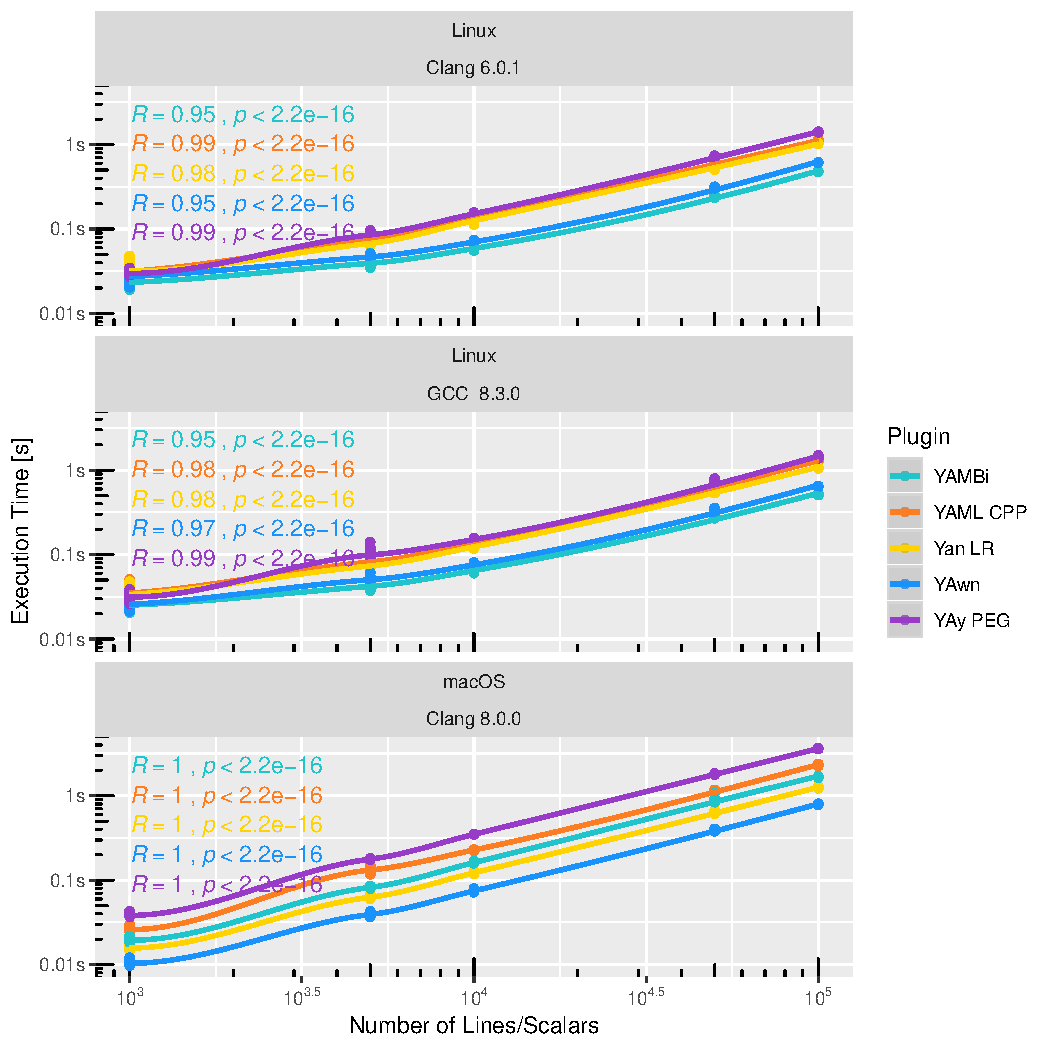
\includegraphics[width=\textwidth]{BenchmarkResultRuntimeAbove1000}
  \caption{The diagrams above shows that the runtime for the first lines of the file \FileGeneratedHundredThousand{} almost certainly grows linearly.}
  \label{fig:benchmark_results_generated_above_1000}
\end{figure}

From the correlation coefficients ($R$) of $0.95$ and higher we deduce that the runtime for all plugins almost certainly grows linearly. This means that the approximate runtime of the plugins should be the same. Now it is time to answer \Cref{que:speed}.

\speed*

The runtime of a non-backtracking recursive descent parser for an \glstext{LL}(1) grammar, as used by YAML CPP, should be $O(n)$. According to the literature the upper boundary for the runtime of

\begin{itemize}
  \item \gls{ALL(*)}, used by Yan LR, is $O(n⁴)$, but the algorithm often performs linearly~\cite[p. 1]{parr2014adaptive},
  \item LALR, used by YAMBi, is $O(n)$~\cite{baxter2017runtime},
  \item an Earley parser, used by YAwn, is $O(n²)$ for unambiguous grammars~\cite[p. 145]{hopcroft1969formal},
  \item a general PEG parsers, as used by YAy PEG, is exponential~\cite[p. 1]{moss2014derivatives} ($O(cⁿ)$) and for PEG parsers that use memoization is $O(n)$~\cite{ford2002packrat}
\end{itemize}

. We now compare the theoretic runtimes with the measured runtimes shown in Figure~\ref{fig:benchmark_results_generated_above_1000}. The text below lists some of our observations.

\begin{itemize}
  \item The deterministic (aka non-backtracking) parsers (YAML CPP, YAMBi) show the expected linear behavior.

  \item Yan LR also executes in linear time for the input. This is probably the result of the relatively simple grammar used by the parser. At least for all our input and test files we also checked that the grammar works with the simpler, but faster \gls{SLL(*)} strategy. This was indeed the case.

  \item YAwn also shows the linear behavior, even though \href{https://github.com/vnmakarov/yaep}{\gls{YAEP}} \href{https://github.com/vnmakarov/yaep/issues/24}{does not implement \citeauthor{leo1991general}’s optimization}~\cite{leo1991general} that makes sure that the algorithm runs in linear time for every \glstext{LR}(k) grammar.

  \item Even YAy PEG’s backtracking parser without memoization show linear behavior. As we already mentioned before in “\nameref{sec:state_of_the_art}” it is generally not clear, if memoization provides runtime improvements for a certain grammar. This seems also one of the reasons, why \gls{PEGTL} does not uses memoization, as can be seen in a quote of Colin Hirsch~\cite{hirsch2016memo}, one of the authors of \gls{PEGTL}, below.

  \begin{quote}
     …it would increase the complexity of the library beyond our design goals and only be useful in a very limited number of cases - in practice packrat parsers often perform worse than simple recursive descent parsers despite being in a better time complexity class.
  \end{quote}

\end{itemize}

Figure~\ref{fig:benchmark_generated} shows that the constant factor between the linear runtimes can be relatively high. For example on macOS, the fastest plugin YAwn is nearly five times faster than the slowest plugin YAy PEG for the file \FileGenerated{}:

\begin{equation}
  \frac{363.2\text{ms}}{73.6\text{ms}} ≅ 4.93
  \label{eq:benchmark_difference}
\end{equation}

. Other interesting observations concerning the runtime are listed below.

\begin{enumerate}
  \item The difference between the runtime of the fastest and slowest plugins for large files is nearly twice as large on macOS.

  \item The OS seems to play a much more important role, than the compiler for all of the used \glstext{YAML} libraries.

  \item While Yan LR and YAwn perform similarly on macOS and Linux, the difference between YAML CPP, YAMBi and YAy PEG on both operating systems can be quite significant.
\end{enumerate}

Since the runtime of the plugins is quite different on the two benchmarked operating systems we also determined mean of the mean values for the file \FileGenerated{}. We use a weight of

\begin{itemize}
  \item $0.5$ for the combination macOS/Clang,
  \item $0.25$ for the combination Linux/Clang, and
  \item $0.25$ for the combination Linux/GCC
\end{itemize}

and obtain the formula:

\begin{equation}
  \overline{t} = 0.5  · \overline{t}_{\text{macOS/Clang}} +
                 0.25 · \overline{t}_{\text{Linux/GCC}} +
                 0.25 · \overline{t}_{\text{Linux/Clang}}
  \label{eq:benchmark_generated_mean}
\end{equation}

. Figure \ref{fig:benchmark_generated_mean} shows a bar graph with the result of this calculation.

\begin{figure}[H]
  \begin{bchart}[max=300, width=0.8\textwidth, unit=ms]

    \bcbar[text=188.9, value=, color=orange]{188.9}

    \bcbar[text=122, value=, color=DarkYellow]{122}

    \bcbar[text=119.9, value=, color=Turquoise3]{119.9}

    \bcbar[text=74.9, value=, color=Aqua]{74.9}

    \bcbar[text=261, value=, color=DarkOrchid]{261}
  \end{bchart}
  \begin{center}
  \vspace{-0.5cm}
    \tikzcircle{orange} YAML CPP ~~
    \tikzcircle{DarkYellow} Yan LR ~~
    \tikzcircle{Turquoise3} YAMBi ~~
    \tikzcircle{Aqua} YAwn ~~
    \tikzcircle{DarkOrchid} YAy PEG
  \vspace{-0.5cm}
  \end{center}
  \caption{This bar chart shows the mean of the mean run times of the plugins according to Equation~\ref{eq:benchmark_generated_mean} for the input \FileGenerated{}.}
  \label{fig:benchmark_generated_mean}
\end{figure}

\subsubsection{Conclusion}

We determined with a high confidence that all of the \glstext{YAML} plugins show a linear runtime behavior (see Figure~\ref{fig:benchmark_results_generated_above_1000}), at least for the file \FileGeneratedHundredThousand{}. This puts all plugins, into the same computational complexity class. The constant difference between the runtime can still be relatively high though, as we can see in Equation~\ref{eq:benchmark_difference}.

The fastest plugin according to the mean of the mean runtimes (see Figure~\ref{fig:benchmark_generated_mean}) is YAwn, if we weigh the results of the two tested operating systems equally. This is interesting, since \citeauthor{earley1970efficient} himself mentions in his dissertation~\cite[p. 122]{earley1970efficient} that his parsing technique was too slow for practical use at the time, as you can see in the quote below.

\begin{quote}
  First we ask, what impact will our algorithm have on the parsing done in production compilers for existing programming languages? The answer is, practically none. Production compilers require guessing time proportional to n with a fairly low coefficient of n.
\end{quote}

Yan LR and YAMBi showed the second best runtimes, and were about $1.6$ times slower than YAwn. YAML CPP, which was, according to the results of Figure~\ref{fig:benchmark_generated_mean}, about $2.5$ times slower than Yawn takes the second to last place. Yay PEG was the slowest plugin on both tested operating systems, and is about $3.5$ times slower than the fastest plugin according to Figure~\ref{fig:benchmark_generated_mean}.

\subsection{Memory Usage}
\label{sec:memory_usage}

\subsubsection{Method}

\newcommand{\FileBenchmarkMemory}{{%
\href{http://rawdata.libelektra.org/tree/master/YAML/Scripts/benchmark-memory}%
{\sh{benchmark-memory}}%
}}

We measured the heap memory usage with the heap profiler \href{http://valgrind.org/docs/manual/ms-manual.html}{Massif}. Most of the other setup is similar to the one we used for the runtime benchmark, described in the section “\nameref{sec:run_time_performance}”. We still use the the C application \FilePluginGetSet{} to execute the plugins. The input files are also the same as before.

This time we do not need to determine the mean value of the results. Massif always produces the same output on the same hardware/software combination, since it runs the instrumented program \FilePluginGetSet{} on a “synthetic CPU”~\cite{valgrind2019core}.

To automate the process of measuring the memory usage for the different input files, we created a Shell script called \FileBenchmarkMemory{}. We only benchmarked the memory usage on Linux, since Massif did not support macOS 10.14 at the time we executed the benchmark script.

\subsubsection{Results}

The graphs in this section show the results of the memory benchmark for different input files.

\begin{figure}[H]
  \begin{bchart}[max=25, width=0.8\textwidth, unit=MB]
    \bcbar[text=17.5, value=Linux/GCC, color=orange]{17.5}
    \bcbar[text=18.3, value=Linux/Clang, color=orange]{18.3}

    \bcbar[text=23.8, value=Linux/GCC, color=DarkYellow]{23.8}
    \bcbar[text=23.8, value=Linux/Clang, color=DarkYellow]{23.8}

    \bcbar[text=10.4, value=Linux/GCC, color=Turquoise3]{10.4}
    \bcbar[text=10.1, value=Linux/Clang, color=Turquoise3]{10.1}

    \bcbar[text=9, value=Linux/GCC, color=Aqua]{9}
    \bcbar[text=8.8, value=Linux/Clang, color=Aqua]{8.8}

    \bcbar[text=22.8, value=Linux/GCC, color=DarkOrchid]{22.8}
    \bcbar[text=23.1, value=Linux/Clang, color=DarkOrchid]{23.1}
  \end{bchart}
  \begin{center}
  \vspace{-0.5cm}
    \tikzcircle{orange} YAML CPP ~~
    \tikzcircle{DarkYellow} Yan LR ~~
    \tikzcircle{Turquoise3} YAMBi ~~
    \tikzcircle{Aqua} YAwn ~~
    \tikzcircle{DarkOrchid} YAy PEG
  \vspace{-0.5cm}
  \end{center}
  \caption{This bar chart shows the peak heap memory usage of the plugins for the input \FileKeyFrames{}.}
  \label{fig:benchmark_memory_keyframes}
\end{figure}

\begin{figure}[H]
  \begin{bchart}[max=25, width=0.8\textwidth, unit=MB]
    \bcbar[text=12.6, value=Linux/GCC, color=orange]{12.6}
    \bcbar[text=12.9, value=Linux/Clang, color=orange]{12.9}

    \bcbar[text=17.5, value=Linux/GCC, color=DarkYellow]{17.5}
    \bcbar[text=17.4, value=Linux/Clang, color=DarkYellow]{17.4}

    \bcbar[text=7.7, value=Linux/GCC, color=Turquoise3]{7.7}
    \bcbar[text=7.6, value=Linux/Clang, color=Turquoise3]{7.6}

    \bcbar[text=7.9, value=Linux/GCC, color=Aqua]{7.9}
    \bcbar[text=7.8, value=Linux/Clang, color=Aqua]{7.8}

    \bcbar[text=14.8, value=Linux/GCC, color=DarkOrchid]{14.8}
    \bcbar[text=14.8, value=Linux/Clang, color=DarkOrchid]{14.8}
  \end{bchart}
  \begin{center}
  \vspace{-0.5cm}
    \tikzcircle{orange} YAML CPP ~~
    \tikzcircle{DarkYellow} Yan LR ~~
    \tikzcircle{Turquoise3} YAMBi ~~
    \tikzcircle{Aqua} YAwn ~~
    \tikzcircle{DarkOrchid} YAy PEG
  \vspace{-0.5cm}
  \end{center}
  \caption{This bar chart shows the peak heap memory usage of the plugins for the input \FileCombined{}.}
  \label{fig:benchmark_memory_combined}
\end{figure}

\begin{figure}[H]
  \begin{bchart}[max=700, width=0.8\textwidth, unit=MB]
    \bcbar[text=526.4, value=Linux/GCC, color=orange]{526.4}
    \bcbar[text=555, value=Linux/Clang, color=orange]{555}

    \bcbar[text=483.5, value=Linux/GCC, color=DarkYellow]{483.5}
    \bcbar[text=480.9, value=Linux/Clang, color=DarkYellow]{480.9}

    \bcbar[text=200.8, value=Linux/GCC, color=Turquoise3]{200.8}
    \bcbar[text=190.3, value=Linux/Clang, color=Turquoise3]{190.3}

    \bcbar[text=164.3, value=Linux/GCC, color=Aqua]{164.3}
    \bcbar[text=156.5, value=Linux/Clang, color=Aqua]{156.5}

    \bcbar[text=668.9, value=Linux/GCC, color=DarkOrchid]{668.9}
    \bcbar[text=684.2, value=Linux/Clang, color=DarkOrchid]{684.2}
  \end{bchart}
  \begin{center}
  \vspace{-0.5cm}
    \tikzcircle{orange} YAML CPP ~~
    \tikzcircle{DarkYellow} Yan LR ~~
    \tikzcircle{Turquoise3} YAMBi ~~
    \tikzcircle{Aqua} YAwn ~~
    \tikzcircle{DarkOrchid} YAy PEG
  \vspace{-0.5cm}
  \end{center}
  \caption{This bar chart shows the peak heap memory usage of the plugins for the input \FileGenerated{}.}
  \label{fig:benchmark_memory_generated}
\end{figure}

\begin{figure}[H]
  \centering
    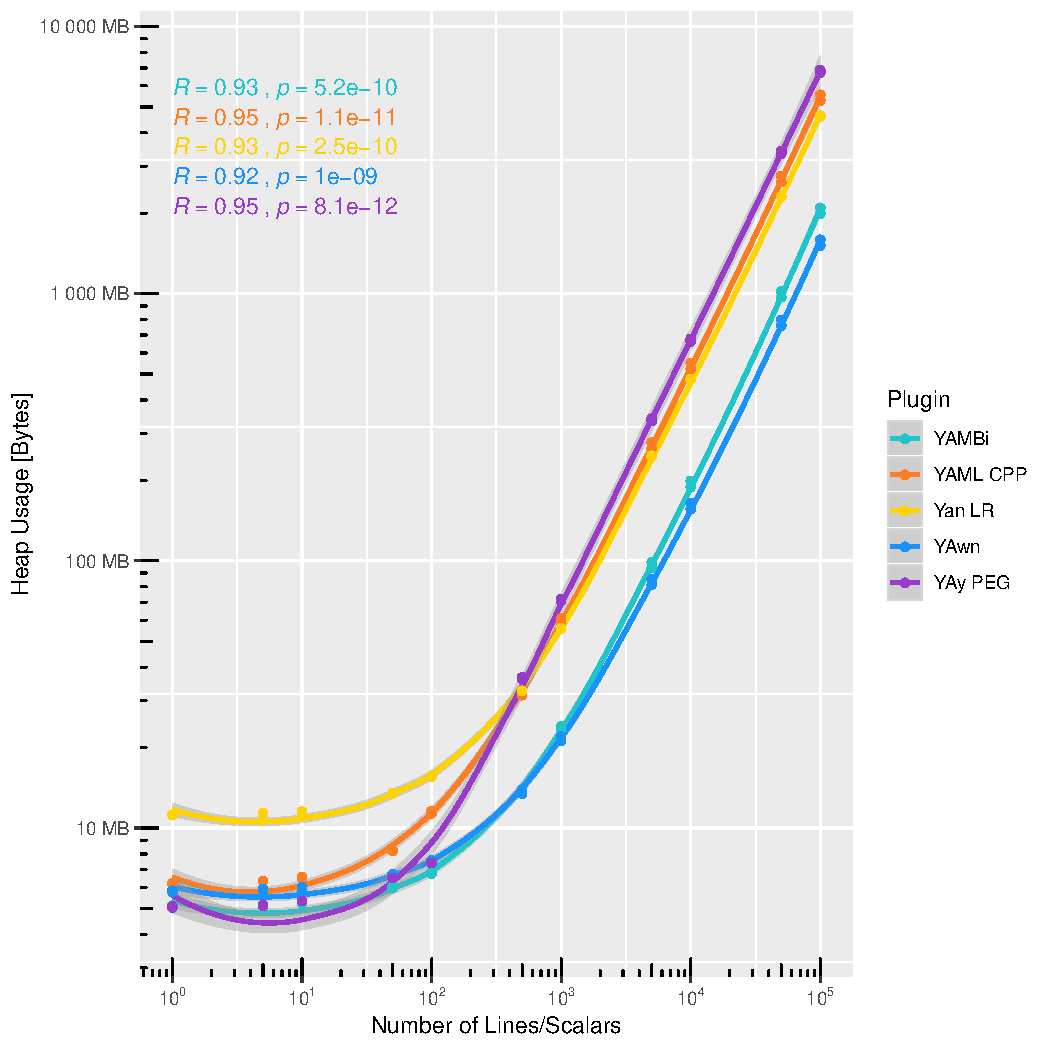
\includegraphics[width=\textwidth]{BenchmarkResultMemory}
  \caption{The diagrams above show the peak heap memory usage of the plugins for the input file \FileGeneratedHundredThousand{} and other files that contain only the first $n$ number of lines of this file.}
  \label{fig:benchmark_results_memory_lines}
\end{figure}

\subsubsection{Analysis}

Figure~\ref{fig:benchmark_results_memory_lines} shows that the memory usage seems to grow linearly for large line numbers. To analyze this behavior further, we limited the data for the graph to observation where the line number is 1000 or higher. Figure~\ref{fig:benchmark_results_memory_lines_above_thousand} shows the graph after this modification. From the correlation coefficients ($R$) of 1 and the low probabilities of the null hypothesis being wrong ($p$) we conclude that the memory consumption almost certainly grows linearly for all plugins.

\begin{figure}[H]
  \centering
    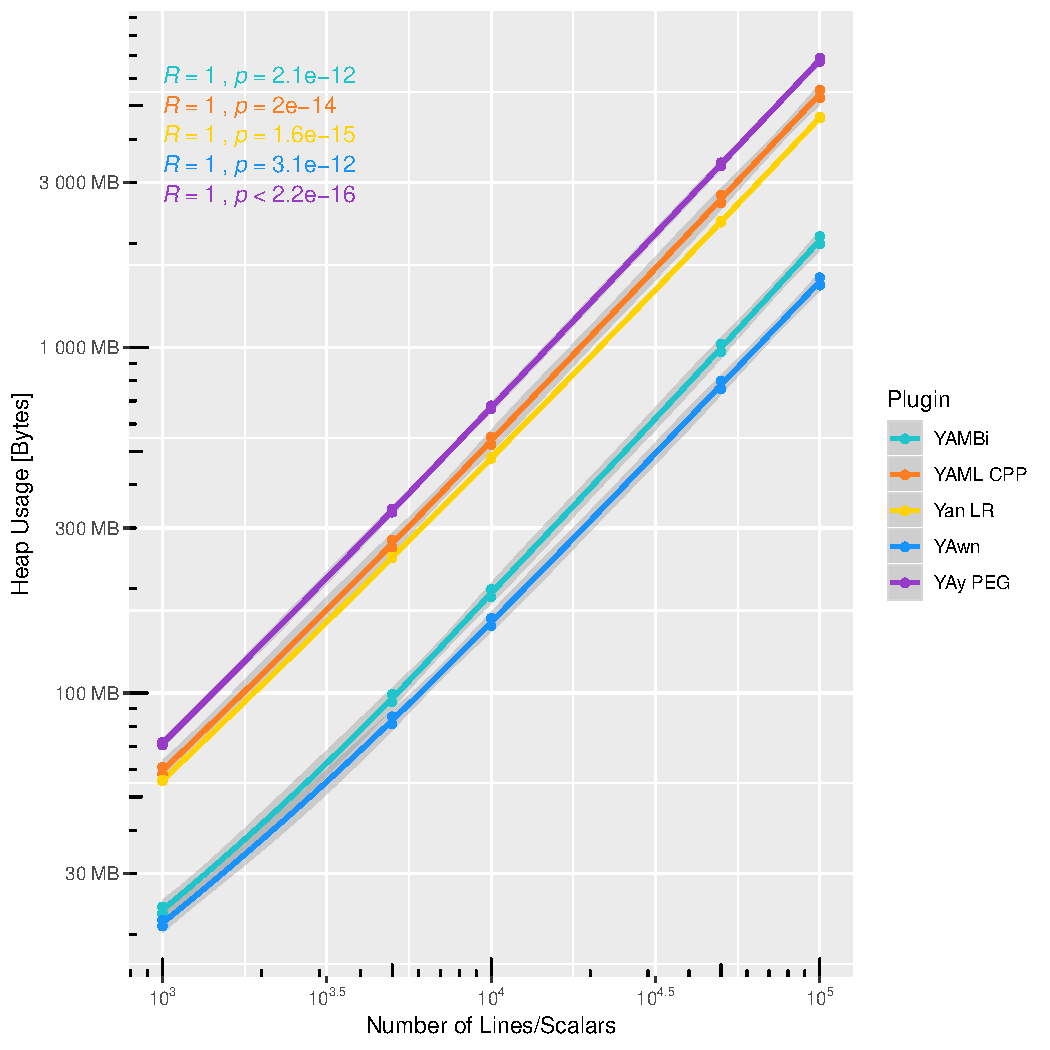
\includegraphics[width=\textwidth]{BenchmarkResultMemoryAbove1000}
  \caption{This diagram above shows that the memory usage of the \glstext{YAML} plugins almost certainly grows linearly for the first $n$ lines of the file \FileGeneratedHundredThousand{}}
  \label{fig:benchmark_results_memory_lines_above_thousand}
\end{figure}

\subsubsection{Conclusion}

While the asymptotic memory usage of all plugins grows linearly according to our measurements, the factor between the memory usage can be quite high. If we look at the data for the file \FileGenerated{} (see Figure~\ref{fig:benchmark_memory_generated}), then YAwn performs best, while YAMBi needs about $20\%$ more heap memory. The memory usage of the other plugins is much worse. Yan LR allocates about three times the heap memory of YAwn, YAML CPP takes about $3.4$ times the memory amount of YAwn, and YAy PEG needs even more than $4$ times the heap memory of YAwn.

\section{Code Size}
\label{sec:code_size}

\subsection{Method}

\newcommand{\FileCountLines}{{%
\codebox{%
\href{http://rawdata.libelektra.org/tree/master/YAML/Scripts/count-lines}%
{\textcolor{black}{\texttt{count-lines}}}}%
}}

We created a Shell script called \FileCountLines{} that counts the code lines of the \glstext{YAML} plugins using the tool \href{https://github.com/AlDanial/cloc}{cloc}. Since cloc \href{http://cloc.sourceforge.net/#Languages}{does not support Bison grammar files}, we wrote code that removes comments and empty lines from a Bison grammar, and afterwards counts the remaining lines using the Unix tool \sh{wc}.

\subsection{Results}

Figure~\ref{fig:line_count} shows the results reported by \FileCountLines{}. As you can see, we did not have to write a grammar for the library based YAML CPP plugin. For the other plugins, we either created a grammar (Yan LR, YAMBi, YAwn), or specified the grammar as handwritten code (Yay PEG). Only the \gls{ANTLR} (Yan LR) and Bison (YAMBi) based plugins use generated code. YAwn, which is based on \gls{YAEP}, uses the grammar directly.

\begin{figure}[H]
  \begin{bchart}[max=2100, width=0.75\textwidth, unit={~Lines of Code}]
    \bcbar[text=609, value=Handwritten, color=orange]{609}

    \bcbar[value=24 ~ Grammar, color=DarkYellow]{24}
    \bcbar[text=717, value=Handwritten, color=DarkYellow]{717}
    \bcbar[text=1108, value=Generated, color=DarkYellow]{1108}

    \bcbar[value=86 ~ Grammar, color=Turquoise3]{86}
    \bcbar[text=766, value=Handwritten, color=Turquoise3]{766}
    \bcbar[text=2046, value=Generated, color=Turquoise3]{2046}

    \bcbar[value=50 ~ Grammar, color=Aqua]{50}
    \bcbar[text=1096, value=Handwritten, color=Aqua]{1096}

    \bcbar[text=1187, value=Handwritten, color=DarkOrchid]{1187}
  \end{bchart}
  \begin{center}
  \vspace{-0.5cm}
    \tikzcircle{orange} YAML CPP ~~
    \tikzcircle{DarkYellow} Yan LR ~~
    \tikzcircle{Turquoise3} YAMBi ~~
    \tikzcircle{Aqua} YAwn ~~
    \tikzcircle{DarkOrchid} YAy PEG
  \vspace{-0.5cm}
  \end{center}
  \caption{This bar chart shows the line counts of of the \glstext{YAML} plugins.}
  \label{fig:line_count}
\end{figure}

\subsection{Analysis}

The line counts of Figure~\ref{fig:line_count} show that YAML CPP requires the least amount of code. That results is not that surprising, considering that the plugin uses yaml-cpp, a library that already represents the \glstext{YAML} file using high-level abstract data structures. We can convert these data structures into Elektra’s \cpp{KeySet} structure relatively easily, keeping the code size of the plugin small.

For a fair size comparison we also have to take the library code itself into consideration. We use the command

\begin{shellcode}
  cloc --include-lang='C++,C/C++ Header' src include
\end{shellcode}

to determine the code size of version 0.6.2 of the yaml-cpp library. The command reports $8413$ lines of code, showing us that parsing the full \glstext{YAML} standard requires a relatively large amount of code.

If we look at the other YAML plugins, we had to write the least code for Yan LR, followed by YAMBi, YAwn, and YAy PEG. The higher line counts of YAMBi and YAwn compared to Yan LR are not that surprising, considering that we implemented some functionality already provided by ANTLR, for those plugins ourselves.

For YAMBi we wrote two classes,

\begin{itemize}
  \item one that represents the input for the lexer ($63$ code lines), and
  \item another class that stores data about a lexer symbol ($53$ code lines)
\end{itemize}

. The sum of the lines of code ($63 + 53 = 116$) explains the difference between the amount of handwritten code between Yan LR and YAMBi ($717 - 609 = 108$) pretty well.

For YAwn we also added a symbol ($69$ code lines) and input class ($101$ code lines) as we did for YAMBi. Additionally we added

\begin{itemize}
  \item tree walking code ($124$ code lines),
  \item a listener ($126$ code lines),
  \item an error listener ($94$ code lines), and
  \item classes storing positional information ($38$ code lines)
\end{itemize}

. The $552$ code lines mentioned above are responsible for about half of the code of the whole plugin ($\frac{1096}{2} = 548$).

YAy PEG, with its scanner-less parsing engine based on C++ templates, uses the most handwritten code. Just like for YAwn we wrote

\begin{itemize}
  \item tree walking code ($128$ lines of code), and
  \item a listener ($122$ lines of code)
\end{itemize}

for the plugin. The other handwritten code take care of parsing ($822$ code lines) and the communication between the plugin and Elektra ($115$ code lines). The amount of parsing code of YAy PEG is quite large, compared to the grammar code of the other plugins. However, we have to consider

\begin{itemize}
  \item that YAy PEG’s parsing code supports a subset of \glstext{YAML} that is a little bit larger, than the one of the lexer based parsing plugins (Yan LR, YAMBi, YAwn), and
  \item that the parsing code also takes care of the work usually done by a lexer
\end{itemize}

. If we look at the lexer based plugins, they use between $352$ (YAMBi) and $416$ (Yan LR) code lines for the lexer.

Handwritten code requires manual work, and is therefore the most interesting criteria when we compare the code size of the plugins. However, the difference between the amount of generated code between the ANTLR based Yan LR plugin ($1108$ code lines), and the Bison based YAMBi plugin ($2046$ code lines) is also interesting. One reason for the big difference might be that ANTLR also requires a runtime library, while Bison generates all code needed for the parser. Both of these approaches have advantages and disadvantages. While Bisons’ approach means no additional dependencies, ANTLR’s runtime library provides space advantages. If multiple programs on the same machine use an ANTLR based parser, they can use the same compiled code, which only has to be stored in memory and on disk once.

\subsection{Conclusion}

If we take the amount of handwritten plugin code as main criteria for the code size comparison, then YAML CPP takes the lead, requiring the least amount of code. This is not surprising, considering that the parsing code of the plugin is part of the external yaml-cpp library, and not part of the plugin code itself.

The parser based plugin with the least amount of code is the ANTLR based Yan LR. The main reason for this is, that ANTLR already generates code for functionality that we had to create ourselves for the other plugins. While writing this support code is usually not that hard, it is certainly an advantage that ANTLR already provides support for common tasks, such as tree walking.

\section{Code Complexity}
\label{sec:code_complexity}

\subsection{Method}

\newcommand{\FileCheckComplexity}{{%
\codebox{%
\href{http://rawdata.libelektra.org/tree/master/YAML/Scripts/measure-complexity}%
{\textcolor{black}{\texttt{measure-complexity}}}}%
}}

For the code complexity analysis we measured the \glsdesc{CC} (\glstext{CC}) of

\begin{itemize}
  \item the parsing libraries and generators,
  \item the generated code (Yan LR, YAMBi), and the
  \item handwritten plugin code
\end{itemize}

with the analyzer \href{http://www.lizard.ws}{lizard}. Since we had to measure the complexity of many different code parts and we wanted to improve the reproducibility of the measurement we created a script for this task called \FileCheckComplexity{}.

\subsection{Results}

Table~\ref{table:cyclomatic_complexity} shows some of the values we measured via \FileCheckComplexity{}.

\begin{table}[H]
  \begin{adjustbox}{max width=\textwidth}
  \begin{threeparttable}
  \caption{The table below shows the measurement results of the script \FileCheckComplexity{}.}
  \label{table:cyclomatic_complexity}
  \centering
  \begin{tabular}{llrrrrrr}
\toprule
     Plugin &                    Part & \glstext{NLOC} & Average \glstext{CC} & Warnings & Function RT & \glstext{NLOC} RT\\
\midrule
   YAML CPP &                yaml-cpp &           7841 &                  2.5 &        7 &        0.01 &              0.09\\
            &                  Plugin &            556 &                  4.6 &        0 &           0 &                 0\\
\midrule
     Yan LR & \gls{ANTLR} C++ Runtime &          15760 &                  2.3 &       18 &        0.01 &              0.15\\
            &                  Plugin &            610 &                  2.1 &        0 &           0 &                 0\\
            &          Generated Code &           1105 &                  1.4 &        0 &           0 &                 0\\
\midrule
      YAMBi &                   Bison &          12677 &                  4.8 &       22 &        0.04 &              0.28\\
            &                  Plugin &            667 &                  2.3 &        0 &           0 &                 0\\
            &          Generated Code &           1526 &                  2.9 &        8 &        0.07 &              0.42\\
\midrule
       YAwn &                    YAEP &           5944 &                  3.9 &       10 &        0.04 &              0.28\\
            &                  Plugin &            990 &                  2.5 &        0 &           0 &                 0\\
\midrule
    YAy PEG &                   PEGTL &           8858 &                  1.6 &        4 &        0.01 &              0.05\\
            &                  Plugin &           1094 &                  2.9 &        0 &           0 &                 0\\
\bottomrule
  \end{tabular}

  \vspace{0.2cm}
  \begin{tablenotes}
    \item
        \hspace{1.65cm}
        \glstext{CC}…\glsdesc{CC}
        \hspace{1.7cm}
        \glstext{NLOC}…\glsdesc{NLOC}
    \item
      \[
       \text{Function RT} = \frac{\text{Warnings}}{\text{Number of Functions}}\quad
       \text{NLOC RT} = \frac{\text{NLOC with Warnings}}{\text{NLOC inside Functions}}
      \]
  \end{tablenotes}

  \end{threeparttable}
  \end{adjustbox}
\end{table}

\subsection{Analysis}

The most interesting parts of Table~\ref{table:cyclomatic_complexity} are the last two columns that show the relative amount of code that has a higher cyclomatic complexity than $15$. None of the handwritten plugin code contains any function with a \gls{CC} over this threshold. This is the result of using the static code analyzer \href{http://oclint.org}{OCLint} to check the code while we developed the plugins. Other than that, only the code generated by \gls{ANTLR} contains no code with a cyclomatic complexity over $15$. The cyclomatic complexity of the generated code by Bison is higher, which does not seem that surprising considering that \glstext{LR} parsers, contrary to \glstext{LL} parser, are almost never written by hand, because of their inherent complexity. If we look at the parser libraries and parser generators themselves, \gls{PEGTL} is the library containing the least amount of code over the complexity threshold, followed by yaml-cpp, and ANTLR’s C++ runtime. Bison and \gls{YAEP} are the generator and library that contain the most code with a high cyclomatic complexity.

\subsection{Conclusion}

While cyclomatic complexity has “never been unambiguously correlated with defective or unmaintainable code”~\cite{martin2017c++}, the measurements in this section provide at least some indication about code that might be problematic due to a high code complexity.

\section{Ease of Extensibility and Composability}
\label{sec:extensibility}

One advantage of parsing libraries and parser generators over handwritten parsers is that we can update the language grammar without having to rewrite parsing code. This way we can extend the parsed \glstext{YAML} subset easily without many manual code changes. In the first part of the next section we analyze how many code line changes it took to, fix bugs in, and add minor features to, the \glstext{YAML} plugins. The amount of code changes provides a good metric on how much effort it takes to extend the parser plugins.

In the second part of this section we will take a look at how the composability of our parsing code influences the extensibility. One option to create an extensible system is to base it on components. We can reuse these components to keep the amount of code for a new feature or bug fix low. We can imagine that the rules of a grammar represent components in our parsing systems. Parsing systems without a separate lexing phase such as PEGTL take the composability idea one step further. In PEGTL we can compose the parser for the whole grammar out of smaller parser that build on each other. We will analyze, if the component based parser of YAy PEG provides extensibility advantages over the other parsers. We will also answer~\Cref{que:closeness} in this part of the thesis.

\closeness*

\subsection{Plugin Updates}

In the next subsections we look at the effort it took to, add certain features to, and fix certain bugs in, the \glstext{YAML} plugins.

\subsubsection{Method}

As measurement for the extendibility effort we use the amount of changed code lines. Since we want to keep the comparison fair, we only look at the code changes needed for a certain feature or bug fix, excluding additional test code and documentation updates.

\subsubsection{Support for Elektra’s Boolean Data Type}

Elektra’s \cc{Key} data structure usually saves data as untyped character string. We can add type information for a certain key by adding a \code{type} meta key (see also Section “\nameref{sec:keyset}”). If we do that Elektra ensures that applications store and retrieve the right kind of data for that specific key. Elektra’s C++ \gls{API} offers a direct way to store and retrieve a typed value via templated functions. We used these functions to improve the support for boolean data types in the \glstext{YAML} plugins.

\glstext{YAML}’s JSON schema represents boolean data as scalar with the canonical value \yaml{false} or \yaml{true}~\cite{ben2009yaml}. More advanced schemas, such as the core schema offer additional aliases for true and false values. For the \glstext{YAML} plugins in this thesis we only added support for the JSON schema though. For this to work we had to translate the \glstext{YAML} values \yaml{false} and \yaml{true} to \href{https://master.libelektra.org/doc/decisions/bool.md}{Elektra’s boolean values} \code{0} and \code{1}.

Just like Elektra’s C++ \gls{API}, yaml-cpp, the library used by the YAML CPP plugin, also offers templated functions to retrieve and set boolean values. One problem of yaml-cpp’s \gls{API} is that there seems to be no way to check for the type of a \glstext{YAML} node, without the possibility of throwing an exception~\cite{beder2013type}. This can be problematic for the runtime efficiency, since YAML CPP might trigger multiple exceptions before it converts a \glstext{YAML} node to a correctly typed Elektra key. To improve the runtime performance of YAML CPP we checked the textual value of a \glstext{YAML} node before we converted it. The implementation of this more \href{https://github.com/ElektraInitiative/libelektra/commit/d4e62eebd006ea4b066c75e6e885ee5a4b6e26cf#diff-4bdb640234f370e3a9db751e1f7d769b}{complicated approach} modified $16$ code lines (\textcolor{Green}{$15$ additions}, \textcolor{Red}{$1$ deletion}), while the implementation of the \href{https://github.com/ElektraInitiative/libelektra/commit/1e9a07baad8a140c6eda654053db450c0901f5d0#diff-4bdb640234f370e3a9db751e1f7d769b}{direct approach} – that might cause more exceptions for data without many boolean values – modified only $9$ additional code lines (\textcolor{Green}{$8$ additions}, \textcolor{Red}{$1$ deletion}).

Adding support for boolean values modified $10$ lines in \href{https://issues.libelektra.org/2653}{Yan LR’s} code base (\textcolor{Green}{$9$ additions}, \textcolor{Red}{$1$ deletion}), and $9$ lines (\textcolor{Green}{$8$ additions}, \textcolor{Red}{$1$ deletion}) in each of the other plugins (\href{https://issues.libelektra.org/2652}{YAMBI}, \href{https://issues.libelektra.org/2651}{YAwn}, \href{https://issues.libelektra.org/2654}{YAy PEG}). The similar line counts are a direct result of all of the plugins using a listener interface to convert parsed \glstext{YAML} data. To add boolean support we only had to change code in one of the functions of the listeners.

\begin{figure}[H]
  \begin{bchart}[max=20, width=0.8\textwidth, unit={~Lines of Code}]
    \bcbar[text=9, value=Direct Approach, color=orange]{9}
    \bcbar[text=16, value=Complex Approach, color=orange]{16}
    \bcbar[text=10, value=, color=DarkYellow]{10}
    \bcbar[text=9, value=, color=Turquoise3]{9}
    \bcbar[text=9, value=, color=Aqua]{9}
    \bcbar[text=9, value=, color=DarkOrchid]{9}
  \end{bchart}
  \begin{center}
  \vspace{-0.5cm}
    \tikzcircle{orange} YAML CPP ~~
    \tikzcircle{DarkYellow} Yan LR ~~
    \tikzcircle{Turquoise3} YAMBi ~~
    \tikzcircle{Aqua} YAwn ~~
    \tikzcircle{DarkOrchid} YAy PEG
  \vspace{-0.5cm}
  \end{center}
  \caption{This bar chart shows the number of modified lines needed for adding better boolean support to the \glstext{YAML} plugins.}
  \label{fig:boolean_line_count}
\end{figure}

\subsubsection{Conversion of Empty Values}

Depending on the context, empty content (empty nodes) in a \glstext{YAML} stream might represent null values. Elektra should store these null values in a key with a zero length binary value. This was not the case in the first version of the parser based \glstext{YAML} plugins (Yan LR, YAMBi, YAwn, YAy PEG). Instead the plugins would incorrectly convert these null values into empty strings.

Another similar problem was that the lexer based plugins would not convert empty content null values right before the end of a file (\code{EOF}\glsadd{EOF}). The result of this bug was that the lexer would not terminate for a stream such as the one shown in Figure~\ref{fig:Figures_StreamNullEOF}.

\begin{figure}[H]
  \centering
    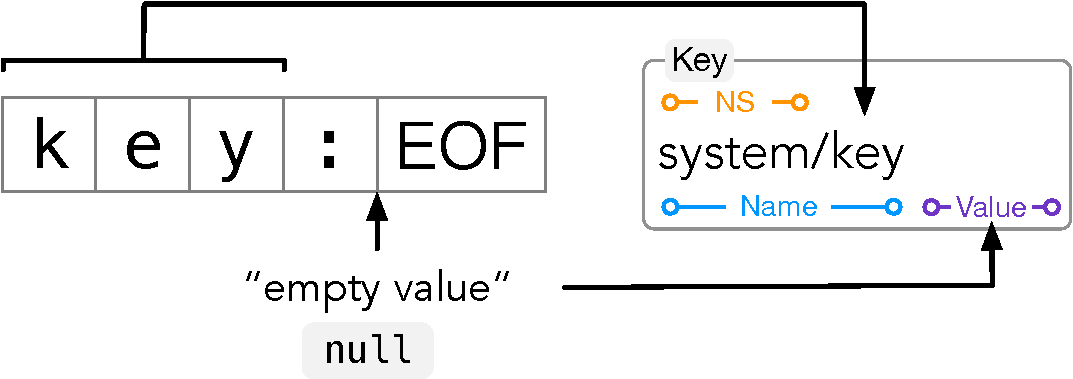
\includegraphics[width=0.75\textwidth]{StreamNullEOF}
  \caption{The \glstext{YAML} data on the left represents a map that contains one key-value pair with the name \code{key} that stores a null value. The \cc{Key} structure on the right shows the converted \glstext{YAML} data, if we store it directly below the \gls{NS} \code{system}.}
  \label{fig:Figures_StreamNullEOF}
\end{figure}

Figure~\ref{fig:null_line_count} shows the amount of changed lines for the \href{https://issues.libelektra.org/2662}{Yan LR}, \href{https://issues.libelektra.org/2663}{YAMBi}, \href{https://issues.libelektra.org/2664}{YAwn}, and \href{https://issues.libelektra.org/2665}{YAy PEG} plugin. The code changes for all the lexer based plugins (Yan LR, YAMBi, YAwn) are almost identical, since we had to fix the problems in the lexer and listener code, which is quite similar for all of those plugins.

For YAy PEG we only had to fix the support for empty nodes in the middle of a \glstext{YAML} stream, since YAy PEG’s parsing code already handled empty nodes at the end of a file correctly. This is probably a direct result of using grammar code that is quite similar to the one from the \href{http://yaml.org/spec/1.2/spec}{YAML specification}. The notable difference between the amount of code we added for the empty node fix (\textcolor{Green}{$5$ additions}, \textcolor{Red}{$1$ deletion}) compared to the one of the lexer based plugins (\textcolor{Green}{$1$ addition}) is also a result of YAy PEG’s grammar. YAy PEG uses the same code path to add empty and non-empty mapping values. The lexer based plugins on the other hand check for an empty value inside the listener code for a key-value pair. We could also use this approach in the YAy PEG plugin, but that would possibly require substantial code changes to the tree walking code.

\begin{figure}[H]
  \begin{bchart}[max=10, width=0.8\textwidth, unit={~Lines of Code}]
    \bcbar[text=1, value=Empty Node, color=DarkYellow]{1}
    \bcbar[text=5, value=Empty Node Before EOF, color=DarkYellow]{5}
    \bcbar[text=1, value=Empty Node, color=Turquoise3]{1}
    \bcbar[text=4, value=Empty Node Before EOF, color=Turquoise3]{4}
    \bcbar[text=1, value=Empty Node, color=Aqua]{1}
    \bcbar[text=4, value=Empty Node Before EOF, color=Aqua]{4}
    \bcbar[text=6, value=Empty Node, color=DarkOrchid]{6}
  \end{bchart}
  \begin{center}
  \vspace{-0.5cm}
    \tikzcircle{orange} YAML CPP ~~
    \tikzcircle{DarkYellow} Yan LR ~~
    \tikzcircle{Turquoise3} YAMBi ~~
    \tikzcircle{Aqua} YAwn ~~
    \tikzcircle{DarkOrchid} YAy PEG
  \vspace{-0.5cm}
  \end{center}
  \caption{This bar chart shows the additional lines needed for fixing the null value support of the \glstext{YAML} plugins.}
  \label{fig:null_line_count}
\end{figure}

\subsubsection{Conversion of Empty Documents}

According to the \glstext{YAML} specification an empty file corresponds to a null value. We did not consider this in the initial versions of the \glstext{YAML} plugins, which meant the empty documents shown in Figure~\ref{fig:null_yaml} were translated incorrectly. Figure~\ref{fig:empty_document_count} shows the amount of code lines we modified to fix this problem for the \href{https://issues.libelektra.org/2711}{Yan LR}, \href{https://issues.libelektra.org/2712}{YAMBi}, \href{https://issues.libelektra.org/2713}{YAwn} and \href{https://issues.libelektra.org/2714}{YAy PEG} plugin.

\begin{figure}[H]
  \centering
  \begin{minipage}[c]{0.48\textwidth}
    \begin{code-boxed}
      \vspace{10pt}
    \end{code-boxed}
  \end{minipage}
  \begin{minipage}[t]{0.02\textwidth}~\end{minipage}
  \begin{minipage}[c]{0.48\textwidth}
    \begin{yamlcode}
      # Empty document
    \end{yamlcode}
  \end{minipage}
  \caption{The examples above show two options on how to store “nothing” (\code{null}) using \glstext{YAML}.}
  \label{fig:null_yaml}
\end{figure}

\begin{figure}[H]
  \begin{bchart}[max=20, width=0.8\textwidth, unit={~Lines of Code}]
    \bcbar[text=10, value=, color=DarkYellow]{10}
    \bcbar[text=17, value=, color=Turquoise3]{17}
    \bcbar[text=15, value=, color=Aqua]{15}
    \bcbar[text=10, value=, color=DarkOrchid]{10}
  \end{bchart}
  \begin{center}
  \vspace{-0.5cm}
    \tikzcircle{orange} YAML CPP ~~
    \tikzcircle{DarkYellow} Yan LR ~~
    \tikzcircle{Turquoise3} YAMBi ~~
    \tikzcircle{Aqua} YAwn ~~
    \tikzcircle{DarkOrchid} YAy PEG
  \vspace{-0.5cm}
  \end{center}
  \caption{This bar chart shows the amount of code lines we modified to fix the conversion of empty documents.}
  \label{fig:empty_document_count}
\end{figure}

\begin{sloppypar}
When we implemented the fixes for the empty document conversion we noticed that we added nearly identical code to the listener (Yan LR, YAwn, YAy PEG) respectively driver (YAMBi) of the plugins. These modifications took \textcolor{Green}{$6$ additions} for Yan LR and \textcolor{Green}{$5$ additions} for the other plugins. We should mention here that we could also have avoided two additional lines for the Yan LR plugin, which consisted of an \cpp{using} statement and the inclusion of an optional header file.
\end{sloppypar}

The other code line differences were a result of grammar updates to

\begin{itemize}
  \item Yan LR (\textcolor{Green}{$3$ additions}, \textcolor{Red}{$1$ deletion}),
  \item YAMBi (\textcolor{Green}{$7$ additions}, \textcolor{Red}{$5$ deletion}), and
  \item YAwn (\textcolor{Green}{$5$ additions}, \textcolor{Red}{$1$ deletion})
\end{itemize}

and updates to tree walking code of:

\begin{itemize}
  \item YAwn (\textcolor{Green}{$4$ additions}), and
  \item YAy PEG (\textcolor{Green}{$5$ additions})
\end{itemize}

. The relatively high number of changes to the grammar of YAMBi is deceiving, since we also moved a 4 line grammar block (\textcolor{Green}{$4$ additions}, \textcolor{Red}{$4$ deletion}) in the bug fix update for the plugin. Figure~\ref{fig:empty_document_minimum_count} takes this code block movement and the optional line changes for Yan LR into account to give a better overview of the code changes we needed to implement the bug fix.

\begin{figure}[H]
  \begin{bchart}[max=20, width=0.8\textwidth, unit={~Lines of Code}]
    \bcbar[text=8, value=, color=DarkYellow]{8}
    \bcbar[text=9, value=, color=Turquoise3]{9}
    \bcbar[text=15, value=, color=Aqua]{15}
    \bcbar[text=10, value=, color=DarkOrchid]{10}
  \end{bchart}
  \begin{center}
  \vspace{-0.5cm}
    \tikzcircle{orange} YAML CPP ~~
    \tikzcircle{DarkYellow} Yan LR ~~
    \tikzcircle{Turquoise3} YAMBi ~~
    \tikzcircle{Aqua} YAwn ~~
    \tikzcircle{DarkOrchid} YAy PEG
  \vspace{-0.5cm}
  \end{center}
  \caption{This bar chart shows the “minimal” code line modifications we needed to fix the conversion of empty documents.}
  \label{fig:empty_document_minimum_count}
\end{figure}

\subsection{Component Based Grammars and Extensibility}

The \href{http://yaml.org/spec/1.2/spec}{YAML specification} includes a detailed grammar description of the language in a parameterized \gls{BNF} like syntax. The grammar rules of the specification are very reminiscent of parser combinator functions~\cite{hutton1992higher, hutton1996monadic}. This is not that surprising considering that \href{https://hackage.haskell.org/package/YamlReference}{YAML’s reference parser} is also based on parser combinators. A large part of the reference parser actually uses slightly modified versions of all of the rules of the \glstext{YAML} spec. Since “the order of alternatives in the grammar is significant”~\cite{ben2009yaml} (ordered choice) and some of the parsing rules also uses positive and negative lookahead we can also categorize \glstext{YAML}’s reference grammar as an extended version of a \gls{PEG}.

In the section “\nameref{sec:peg_parser}” we already mentioned that the grammar description of the YAy PEG plugin resembles the \glstext{YAML} specification grammar quite closely. It is time to analyze, if this close resemblance provides advantages over the other \glstext{YAML} plugins, which use a description that is quite different to the one of the \glstext{YAML} specification.

Table~\ref{table:extensibility} lists some of the advantages and disadvantages we found while we implemented and extended the \glstext{YAML} plugins.

\begin{table}[H]
  \caption{The table below lists some advantage and disadvantages of PEG based (YAy PEG) and lexer based (Yan LR, YAMBi, YAwn) plugins regarding extensibility.}
  \label{table:extensibility}
  \centering
  \begin{tabular}{ll}
\toprule
                           \tikzcircle{DarkOrchid} YAy PEG & \tikzcircle{DarkYellow} \tikzcircle{Turquoise3} \tikzcircle{Aqua} Lexer Based Plugins\\
\midrule
\textcolor{Green}{+} Grammar Extension via “Copy \& Paste” &                                 \textcolor{Green}{+}                   Simple Grammar\\
                    \textcolor{Red}{–} Complicated Grammar &                                                 \textcolor{Red}{–} Handwritten Lexer\\
                              \textcolor{Red}{–} Debugging &                                                                                      \\
\bottomrule
  \end{tabular}
\end{table}

Using the PEG library certainly offers advantages considering the extensibility of the grammar, since we can more or less copy the grammar rules from the specification or reference parser and modify them slightly for \gls{PEGTL}. Fortunately the reference parser already contains a relatively large test suite, which means the chance of errors in the reference grammar is quite low. This is helpful, since the specification grammar consists of 211 rules, which can be quite complicated. This is also one of the disadvantages of using \gls{PEGTL}, since the grammar of YAy PEG is more complicated than the one of the lexer based plugins. The complexity is a result of using a single pass to parse \glstext{YAML} data instead of using a separate lexer and parser phase. The single parsing phase also makes debugging harder since we can not debug the lexer and parsing code separately.

Keeping the information above in mind we can now answer \Cref{que:closeness}.

  \closeness*

The parser of YAy PEG certainly stays closest to the grammar definition of the \glstext{YAML} specification. This closeness is helpful, if we look at the extension of the grammar. However, since YAy PEG’s grammar code also handles low level details of the parsing process we have to consider these details later in the parsing process, which reduces the extensibility of the parsing support code compared to the one of the lexer based plugins.

\subsection{Conclusion}

The examples at the start of this section show that the extensibility of the different \glstext{YAML} plugins depend on the specific bug we want to fix or the feature we like to add. Sometimes the code changes can be quite similar, at least for all the lexer based plugins (Yan LR, YAMBi, YAwn). Other times we need to change code in nearly all parts of a plugin. In these cases plugins that use generators and libraries that provide more built-in code support are easier to extend. If we take the built-in support code into account, then the order of ease of extensibility for the lexer based plugins is roughly Yan LR, followed by YAMBi and then YAwn.

YAML CPP’s extensibility depends on the specific part we need to extend. While we can modify the conversion code of the plugin easily, fixing bugs in the lexer or adding features, such as comment preservation would require us to change the library code of yaml-cpp. This would take more effort, than it would for the the other \glstext{YAML} plugins for a similar feature, since we would have to update yaml-cpp’s handwritten parser code instead of the code of a more compact grammar file.

YAy PEG’s advantage considering grammar extensibility is that the plugin uses parsing code that is very similar to the one of the \glstext{YAML} specification. This allows us to extend the grammar relatively easily by taking rules from the \glstext{YAML} specification and modifying them slightly. The similarity of the grammar code can also be a disadvantage though, since the support code of the plugin needs to consider the many rules of the specification grammar compared to the relatively simple grammar rules of the lexer based plugins.

\section{Error Reporting}
\label{sec:error_reporting}

While there exist techniques to enhance error reporting, by using external tools or modifying a parser engine (see Section “\nameref{sec:error_handling}”), we will only consider built-in solutions or slight modifications to a grammar. We do this, since extending a parser engine is out of scope of the thesis and elaborate extensions would also make the comparison concerning error reporting unfair.

\subsection{Initial Erroneous Input}

Listing \ref{lst:list_element_outside} shows the erroneous \glstext{YAML} data we used initially to compare the error reporting capabilities. Listing~\ref{lst:list_element_inside} and \ref{lst:list_element_removed} show two solutions to fix the problematic part of the \glstext{YAML} document.

\begin{listing}
  \begin{code-boxed}
    \inputminted[linenos]{yaml}{Data/Errors/list_element_outside.yaml}
  \end{code-boxed}
  \caption{The indentation of the sequence item \yaml{- element 2} is incorrect in the code above. One of the most obvious solutions to fix the syntax error would be to add a single space character right before \yaml{- element 2} (see Listing~\ref{lst:list_element_inside}). Another solution is to remove \yaml{- element 2} altogether (see Listing~\ref{lst:list_element_removed}).}
  \label{lst:list_element_outside}
\end{listing}

\begin{listing}
  \begin{code-boxed}
    \inputminted[linenos]{yaml}{Data/Correct/list_element_inside.yaml}
  \end{code-boxed}
  \caption{Usually a person would fix the error shown in Listing~\ref{lst:list_element_outside} by adding an indentation character before the sequence item \yaml{- element 2}.}
  \label{lst:list_element_inside}
\end{listing}

\begin{listing}
  \begin{code-boxed}
    \inputminted[linenos]{yaml}{Data/Correct/list_element_removed.yaml}
  \end{code-boxed}
  \caption{One of the easiest solutions to fix the code in Listing~\ref{lst:list_element_outside} for a computer program is to remove \yaml{- element 2}.}
  \label{lst:list_element_removed}
\end{listing}

\subsection{Basic Error Messages}

We started the comparison by listing the basic error messages for the \glstext{YAML} plugins. These messages contain the error location and the auto-generated error message by the parsing engines. For the sake of brevity we removed data that is identical for all plugins, such as the filename of the parsed file.

\begin{table}
  \caption{Basic error messages}
  \label{tab:error_messages_list_element_outside}
  \centering
  \begin{tabular}{llp{10cm}}
    \toprule
    Plugin & Parser & Message\\
    \midrule
    YAML CPP &
    yaml-cpp &
    yaml-cpp: error at line 3, column 1: end of map not found\\

    Yan LR &
    ANTLR &
    3:1: mismatched input \textquotesingle- \textquotesingle\ expecting BLOCK\_END\\

    YAMBi &
    Bison &
    3:1: syntax error, unexpected ELEMENT, \newline
    expecting KEY or BLOCK\_END\\

    YAwn &
    YAEP &
    3:1: Syntax error on token number 9: \newline
    “<Token, ELEMENT, -, 3:1–3:2>”\\

    YAy PEG &
    PEGTL &
    3:0(18): parse error matching tao::yaypeg::eof\\
    \bottomrule
  \end{tabular}
\end{table}

\subsubsection{Interpretation}

As we can see in Table~\ref{tab:error_messages_list_element_outside} all of the parsing engines report the error location for the code from Listing~\ref{lst:list_element_outside} correctly. The error messages also shows that the question, if the first position after a newline is at column 0 or 1, is still open for debate. Other than that we can see that YAML CPP, Yan LR, and YAMBi also show information about the expected element at the error position (end of a block \gls{collection} is missing). YAML CPP provides the best error message, since the plugin also shows which type of end element is missing (end of map). This type of information can also be determined easily in all of the lexer-based parsing engine plugins (Yan LR, YAMBi, YAwn). We modified them accordingly. Table~\ref{tab:error_messages_improved_list_element_outside} shows the slightly improved error messages, highlighting the updated part of the text.

\begin{table}
  \caption{Slightly improved error messages}
  \label{tab:error_messages_improved_list_element_outside}
  \centering
  \begin{tabular}{llp{10cm}}
    \toprule
    Plugin & Parser & Message\\
    \midrule
    YAML CPP &
    yaml-cpp &
    yaml-cpp: error at line 3, column 1: end of map not found\\

    Yan LR &
    ANTLR &
    3:1: mismatched input \textquotesingle- \textquotesingle\ expecting \textbf{MAP\_END}\\

    YAMBi &
    Bison &
    3:1: syntax error, unexpected ELEMENT, \newline
    expecting \textbf{MAP\_END} or KEY\\

    YAwn &
    YAEP &
    3:1: Syntax error on token number 9: \newline
    “<Token, ELEMENT, -, 3:1–3:2>”\\

    YAy PEG &
    PEGTL &
    3:0(18): parse error matching tao::yaypeg::eof\\
    \bottomrule
  \end{tabular}
\end{table}

After the slight modifications to the \glstext{YAML} parser plugins we decided to take a closer look at the error handling capabilities of each of the parsing engines on their own in the next subsections.

\subsection{ANTLR}

ANTLR uses an error listener class that provides a callback method that includes access to

\begin{itemize}
  \item the location,
  \item the offending symbol,
  \item the used recognizer class,
  \item the thrown exception, and
  \item the default error message
\end{itemize}

for each detected error. As we already saw in Table~\ref{tab:error_messages_improved_list_element_outside}, the default error message provided by ANTLR usually describes errors already well. For the initial version of the \href{http://libelektra.org/plugins/yanlr}{Yan LR plugin}, we only stored the last error message reported by ANTLR. Since ANTLR uses methods such as token deletion and insertion to keep parsing a file, even if it contains multiple errors~\cite{parr2013definitive}, the last error message usually will not provide the the most obvious information on how to fix an error.

\begin{listing}
  \begin{minted}[autogobble, linenos]{yaml}
    key: - element 1
      - element 2 # Incorrect Indentation!
  \end{minted}
  \caption{The indentation of the sequence element \yaml{- element 2} is incorrect in the code above.}
  \label{lst:incorrect_indentation}
\end{listing}

For example, for the input shown in Listing~\ref{lst:incorrect_indentation} the parser produced the following error output:

\begin{textcode}
  2:37: extraneous input 'MAP END' expecting {STREAM_END, COMMENT}
\end{textcode}

. To fix this defect in the Yan LR plugin, we stored all error messages which resulted in the better error report:

\begin{textcode}
  2:1: mismatched input '- ' expecting MAP_END
  2:37: extraneous input 'MAP END' expecting STREAM_END
\end{textcode}

. You might also notice that in the error report \code{COMMENT} is missing from the list of expected tokens. This difference is the result of an \href{https://github.com/ElektraInitiative/libelektra/commit/0fe4953}{ambiguity in the ANTLR grammar we fixed}.

One of the more recent improvements in error messages of modern compilers such as Clang and GCC is the ability to highlight erroneous input. We also implemented this error reporting mechanism based on the Java code in \citetitle[page 158]{parr2013definitive}~\cite{parr2013definitive}. The text:

\begin{textcode}
2:1: mismatched input '- ' expecting MAP_END
     - element 2 # Incorrect Indentation!
     ^^
2:37: extraneous input 'MAP END' expecting STREAM_END
      - element 2 # Incorrect Indentation!
                                          ^
\end{textcode}

shows the improved error message for Listing~\ref{lst:incorrect_indentation}. One thing that this error report still lacks is a more human friendly representation of the tokens. Someone with limited knowledge of the \glstext{YAML} specification and Yan LR’s lexer code will probably not know what \code{MAP\_END}, \code{MAP END} and \code{STREAM\_END} mean. One option to improve this situation is to replace the text used by the lexer (\code{MAP END}) and the parser (\code{MAP\_END}, \code{STREAM\_END}). The update of the relevant lexer code is trivial, since we can create tokens containing arbitrary text. For the parser code generated by ANLTR, we used a script that uses regular expressions to replace the relevant strings such as \cc{"MAP_END"} and \cc{"STREAM_END"}. After this update the error report for the \glstext{YAML} data in Listing~\ref{lst:incorrect_indentation} looks like this:

\begin{textcode}
2:1: mismatched input '- ' expecting end of map
     - element 2 # Incorrect Indentation!
     ^^
2:37: extraneous input 'end of map' expecting end of document
      - element 2 # Incorrect Indentation!
                                          ^
\end{textcode}

.

\subsection{Bison}

In the first improvement step for the error messages of the Bison parser, we defined alternative names for tokens, just like we did for Yan LR. Bison supports this feature directly, which means we did not have to write a script to replace the symbols in the generated parser code. After this update the error message from Table~\ref{tab:error_messages_improved_list_element_outside} changed from:

\begin{textcode}
  3:1: syntax error, unexpected ELEMENT, expecting MAP_END or KEY
\end{textcode}

to

\begin{textcode}
  3:1: syntax error, unexpected element, expecting end of map or key
\end{textcode}

.

We then looked into the error recovery capabilities of Bison. Unlike ANTLR the generated parser does not do error recovery by default, but rather exits on the first error. To improve the error behavior, Bison offers the possibility to add the predefined \code{error} token to a grammar. Every time the Bison parser encounters an error it will produce this token~\cite{donnelly2019bison}. We modified the grammar to allow errors inside \glstext{YAML} maps and sequences:

\begin{ccode}
  pairs : pair
        | pairs pair
        | pairs error /* Allow errors after key-value pairs */
        ;

  elements : element
           | elements element
           /* Allow errors after elements of a sequence */
           | elements error
           ;
\end{ccode}

. This way the parser is able to report multiple syntax errors.

\begin{listing}
  \begin{minted}[autogobble, linenos]{yaml}
    key 1: - element 1
     - element 2
    key 2: scalar
           - element 3
  \end{minted}
  \caption{The indentation of the sequence item \yaml{- element 2} is incorrect in the code above. Another error is that the value of \yaml{key 2} can not be both a scalar (\yaml{scalar}) and a sequence (containing \yaml{- element 3}).}
  \label{lst:incorrect_indentation_element_without_sequence}
\end{listing}

After the update the parser produces an error message that looks like this:

\begin{textcode}
2:2: unexpected start of sequence, expecting end of map or key
      - element 2
      ^
4:8: unexpected start of sequence, expecting end of map or key
            - element 3
            ^
\end{textcode}

for the input shown in Listing~\ref{lst:incorrect_indentation_element_without_sequence}. As you can see above, we also added the erroneous input to the error message, just like we did in the Yan LR plugin.

\subsection{YAEP}

Just as Bison, \gls{YAEP} also requires that we add error tokens to the grammar to specify locations for error recovery. We therefore defined the same error recovery locations inside sequences and maps, as we did for Bison. The other updates were quite similar too: We improved the name of tokens inside error messages and added the erroneous input to the error message.

After all these changes the output for the \glstext{YAML} data from Listing~\ref{lst:incorrect_indentation_element_without_sequence} looks very similar to the one produced by YAMBi:

\begin{textcode}
2:2: Syntax error on input “start of sequence”
      - element 2
      ^
4:8: Syntax error on input “start of sequence”
            - element 3
            ^
\end{textcode}

. The only thing missing is the information about the expected type of token.

\subsection{PEGTL}

We already talked about general error strategies for \glstext{PEG} parsers in the Section “\nameref{sec:error_handling}”. PEGTL does neither implement the error handling strategy described by \citeauthor{ford2002packrat}~\cite{ford2002packrat}, nor labelled failures~\cite{maidl2016labeled}. Instead the library offers a grammar rule called \cpp{must}, which states that a certain rule, specified as template argument, has to match at a given position or an error will be raised. We can customize the code executed for a given \cpp{must} rule according to this template argument. Effectively this strategy allows us to specify different error messages for each expected but unmatched rule.

As we described in the section “\nameref{sec:peg_parser}”, we tried to keep the grammar of our PEG parser plugin \href{https://libelektra.org/plugins/yaypeg}{YAy PEG} close to the grammar of the \href{http://yaml.org/spec/1.2/spec}{YAML specification}~\cite{ben2009yaml}. This also meant, that the grammar contained only a single \cpp{must} rule, that makes sure that the grammar matched the whole input:

\begin{cppcode}
  struct yaml : if_must<l_yaml_stream, eof> {};
\end{cppcode}

. The code above also explains the initial version of the error message shown in Table~\ref{tab:error_messages_improved_list_element_outside}:

\begin{textcode}
  3:0(18): parse error matching tao::yaypeg::eof
\end{textcode}

, which tells us, that the parser was unable to match the expected “end of file” in line 3 of the input. We customized the error message above to show a more user friendly text:

\begin{textcode}
  3:0: Incomplete document, expected “end of file”
       - element 2
       ^
\end{textcode}

. As you can see we also added the erroneous input to the message, just as we did for the other parsing engines.

The same single error message, regardless of the error, is not helpful. For good error reporting we need to add other \cpp{must} rules. However, adding failure points (\cpp{must} rules) changes the behavior of the grammar and might even cause the parser to fail on valid input. To minimize the probability of incorrect grammar changes we only added a few rules for situation we were sure that the remainder of a grammar rule had to match. For example, when the parser reads an unescaped single or double quote character (outside of a block scalar) at the beginning of a line or after a whitespace character, it found a quoted flow scalar. Therefore

\begin{enumerate}
  \item the text after the initial quote has to be followed by a (possibly empty) text containing only certain characters, and
  \item the last character of the flow scalar has to be an unescaped quote
\end{enumerate}

. If one of those two rules is not fulfilled, then the parser found a syntax error. After we updated the code accordingly the error message for the \glstext{YAML} data

\begin{yamlcode}
  "double quoted
\end{yamlcode}

looks like this:

\begin{textcode}
  1:14: Missing closing double quote or
        incorrect value inside flow scalar
        "double quoted
                      ^
\end{textcode}

. As you may have noticed we included both error possibilities in the error message, since reacting to both errors independently would require fundamental changes to the grammar.

\subsection{Final Error Messages}

\subsubsection{Element Outside of Sequence}

Table~\ref{tab:error_messages_final_list_element_outside} shows the final error messages for the code of Listing~\ref{lst:list_element_outside}:

\begin{code-boxed}
  \inputminted[linenos]{yaml}{Data/Errors/list_element_outside.yaml}
\end{code-boxed}

.

\begin{table}[H]
  \caption{Final error messages for the \glstext{YAML} code of Listing~\ref{lst:list_element_outside}}
  \label{tab:error_messages_final_list_element_outside}

  \centering
  \begin{tabular}{lp{0.8\textwidth}}
    \toprule
    Plugin & Error Messages\\
    \midrule

    \vspace{0cm}
    YAML CPP &
    \vspace{-0.36cm}
    \begin{textcode}
      error at line 3, column 1: end of map not found.
    \end{textcode}
    \\

    \vspace{0cm}
    Yan LR &
    \vspace{-0.36cm}
    \begin{textcode}
      3:1: mismatched input '- ' expecting end of map
           - element 2
           ^^
    \end{textcode}
    \\

    \vspace{0cm}
    YAMBi &
    \vspace{-0.36cm}
    \begin{textcode}
      3:1: syntax error, unexpected element,
           expecting end of map or key
           - element 2
           ^^
    \end{textcode}
    \\

    \vspace{0cm}
    YAwn &
    \vspace{-0.36cm}
    \begin{textcode}
      3:1: Syntax error on input “-”
           - element 2
           ^^
    \end{textcode}
    \\

    \vspace{0cm}
    YAy PEG &
    \vspace{-0.36cm}
    \begin{textcode}
      3:0: Incomplete document, expected “end of file”
           - element 2
           ^
    \end{textcode}
    \\

    \bottomrule

  \end{tabular}
\end{table}

\paragraph{Interpretation}

\begin{itemize}
  \item All the parsing engines report the correct error location.
  \item YAy PEG and YAwn do not tell us in which \glstext{YAML} node the error occurs. All the other plugins report that a map ended prematurely.
  \item The error message of YAMBi reports an additional option – besides deleting the input – to fix the error: adding a key (in the line between \yaml{- element 1} and \yaml{- element 2}).
\end{itemize}

The list below shows a ranking of the plugins according to the interpretation of the error messages above.

\begin{enumerate}
  \item YAMBi
  \item \glstext{YAML} CPP, Yan LR
  \item YAy PEG, YAwn
\end{enumerate}

\subsubsection{\glstext{YAML} Data Containing Multiple Errors}

The \glstext{YAML} data from Listing~\ref{lst:list_element_outside} only contains a single syntax error. To compare the error recovery capabilities of the parsing libraries, we used \glstext{YAML} data that contains multiple syntax errors as input (see Listing~\ref{lst:multiple_errors}).

\begin{listing}
  \begin{code-boxed}
    \inputminted[linenos]{yaml}{Data/Errors/multiple_errors.yaml}
  \end{code-boxed}
  \caption{The \glstext{YAML} data above contains three syntax errors that we directly describe in the comments right next to the error positions.}
  \label{lst:multiple_errors}
\end{listing}

Table~\ref{tab:error_messages_final_multiple_errors} shows the error messages of the different storage plugins for the \glstext{YAML} input of Listing~\ref{lst:multiple_errors}. As we can see the error output is quite different.

\begin{table}[H]
  \caption{Error messages for the \glstext{YAML} code of Listing~\ref{lst:multiple_errors}}
  \label{tab:error_messages_final_multiple_errors}
  \centering

  \begin{adjustbox}{max width=\textwidth}
  \begin{tabular}{lp{0.86\textwidth}}
    \toprule
    Plugin & Error Messages\\
    \midrule

    \vspace{0cm}
    YAML CPP &
    \vspace{-0.36cm}
    \begin{textcode}
      error at line 5, column 5: end of map not found.
    \end{textcode}
    \\

    \vspace{0cm}
    Yan LR &
    \vspace{-0.36cm}
    \begin{textcode}
      5:5: mismatched input 'element 3' expecting end of sequence
               element 3 # Missing `- `
               ^^^^^^^^^
      6:1: extraneous input 'end of sequence' expecting end of map
           key 3: "double quoted scalar"
           ^
      11:4: mismatched input 'start of map' expecting end of map
               key 6: # Not on same level as key 5
               ^
      13:1: mismatched input 'end of map' expecting end of document
            key 7: 'single quoted scalar'
            ^
    \end{textcode}
    \\

    \vspace{0cm}
    YAMBi &
    \vspace{-0.36cm}
    \begin{textcode}
      5:5: syntax error, unexpected plain scalar,
           expecting end of sequence or element
               element 3 # Missing `- `
               ^^^^^^^^^
      11:4: syntax error, unexpected start of map,
            expecting end of map or key
               key 6: # Not on same level as key 5
               ^
      13:1: syntax error, unexpected key, expecting end of document
            key 7: 'single quoted scalar'
            ^
    \end{textcode}
    \\

    \vspace{0cm}
    YAwn &
    \vspace{-0.36cm}
    \begin{textcode}
      5:5: Syntax error on input “element 3”
               element 3 # Missing `- `
               ^^^^^^^^^
      11:4: Syntax error on input “start of map”
               key 6: # Not on same level as key 5
               ^
      13:1: Syntax error on input “key”
            key 7: 'single quoted scalar'
            ^
      16:1: Syntax error on input “scalar”
            scalar # Not a key
            ^^^^^^
    \end{textcode}
    \\

    \vspace{0cm}
    YAy PEG &
    \vspace{-0.36cm}
    \begin{textcode}
      5:0: Incomplete document, expected “end of file”
               element 3 # Missing `- `
           ^
    \end{textcode}
    \\

    \bottomrule

  \end{tabular}
  \end{adjustbox}

\end{table}

\paragraph{Interpretation}

\begin{itemize}

  \item \emph{YAML CPP} and \emph{YAy PEG} do not provide any error recovery.

  \item \emph{YAy PEG} shows the correct line number for the first error, but not the the correct column number. The plugin also only provides a very generic error message.

  \item All of the plugins that use error recovery (Yan LR, YAMBi, YAwn) print a spurious error messages about an error at line 13.

  \item \emph{Yan LR} shows two error messages for the first syntax error, and one for the second syntax error. Error messages one and three describe the problematic part of the \glstext{YAML} data reasonably well.

  \item Compared to Yan LR, \emph{YAMBi’s} (non-spurious) error messages also describe a second option to fix the erroneous input. However, while the first error message provides a useful suggestion on how to fix the error (insertion of a sequence element), the second option in the second error messages (insertion of a key), will probably confuse anyone that does not know how YAMBi’s lexer works.

  \item \emph{YAwn} prints the same error messages as YAMBi, without the crucial information about the expected element. In addition YAwn prints a fourth error message that addresses the third syntax error.

\end{itemize}

According to the interpretation we concluded that all of the plugins with error recovery provide about the same level of useful error information. YAML CPP describes the first error reasonably well, while the error message from YAy PEG is not that useful. This leaves us with the following ranking of the error capabilities of the plugins based on the input of Listing~\ref{lst:multiple_errors}:

\begin{enumerate}
  \item Yan LR, YAMBi, Yawn
  \item YAML CPP
  \item YAy PEG
\end{enumerate}

.

\subsection{Conclusion}

While the parsing libraries do not produce particularly great error messages, at least the ANTLR (Yan LR) and Bison (YAMBi) plugin, provide error messages that are comparable in quality to the ones of the handwritten parsing engine (YAML CPP).

One advantage of Yan LR, YAMBi, and YAwn is that their parsers offer error recovery. They are therefore able to report multiple errors in a file. This is something that YAML CPP is currently not able to do. ANTLR offers error recovery for free, while Bison and YAEP require the addition of error tokens to the grammar. This can be problematic, since these error tokens can produce conflicts in the case of Bison, and ambiguous parsing results in the case of YAEP.

The parsing plugin that showed the least useful error messages is YAy PEG. While the PEGTL offers basic error handling facilities that are able to provide good error messages for character level errors, producing good error messages for “high-level” errors would probably require a substantial amount of work.

\section{Most Promising Plugin}

Using the information we collected in this chapter it is time to determine the most promising \glstext{YAML} plugin. Let us start by saying that we think all of the parser based \glstext{YAML} plugins (Yan LR, YAMBi, YAwn, YAy PEG) could be extended to parse a more complete subset of \glstext{YAML}. However, some of them fit all the requirements we have for a more complete \glstext{YAML} plugin better than others. Since the whole evaluation is quite extensive we summarize general information about the used parser libraries in Table~\ref{tab:parser_overview} and the concrete parsing plugins in Table~\ref{tab:plugin_overview}.

\begin{table}[H]
  \caption{Overview of the used parsing libraries and their characteristics}
  \label{tab:parser_overview}
  \centering

  \begin{adjustbox}{max width=\textwidth}
  \begin{threeparttable}
  \begin{tabular}{p{2cm}p{2.3cm}p{2.3cm}p{2.3cm}p{2.3cm}p{2.3cm}}
    \toprule
    & \href{https://github.com/jbeder/yaml-cpp}{yaml-cpp} & \href{http://antlr.org}{ANTLR} & \href{https://www.gnu.org/software/bison}{Bison} & \href{https://github.com/vnmakarov/yaep}{YAEP} & \href{https://github.com/taocpp/PEGTL}{PEGTL}\\
    \midrule

    Parser \newline Techniques &
    \begin{minipage}[t]{\linewidth}
    \begin{itemize}[leftmargin=*, itemsep=-1ex]
      \item Recursive Descent
    \end{itemize}
    \end{minipage}
    &
    \begin{minipage}[t]{\linewidth}
    \begin{itemize}[leftmargin=*, itemsep=-1ex]
      \item \glstext{SLL(*)}
      \item \glstext{ALL(*)}
    \end{itemize}
    \end{minipage}
    &
    \begin{minipage}[t]{\linewidth}
      \begin{itemize}[leftmargin=*, itemsep=-1ex]
      \item \glstext{LALR}
      \item \glstext{IELR}
      \item \glstext{LR}
      \item \glstext{GLR}
    \end{itemize}
    \end{minipage}
    &
    \begin{minipage}[t]{\linewidth}
      \begin{itemize}[leftmargin=*, itemsep=-1ex]
      \item Earley Parser
    \end{itemize}
    \end{minipage}
    &
    \begin{minipage}[t]{\linewidth}
      \begin{itemize}[leftmargin=*, itemsep=-1ex]
      \item \glstext{PEG} Parser
    \end{itemize}
    \end{minipage}
    \\

    Lexer \newline Support & Handwritten & Integrated (Regex) & External & External & Integrated (\glstext{PEG})\\

    Grammar
    &
    C++ Code
    &
    \begin{minipage}[t]{\linewidth}
    \begin{itemize}[leftmargin=*, itemsep=-1ex]
      \item Standalone
      \item Annotated with Code
    \end{itemize}
    \end{minipage}
    &
    \begin{minipage}[t]{\linewidth}
    \begin{itemize}[leftmargin=*, itemsep=-1ex]
      \item Annotated with Code
    \end{itemize}
    \end{minipage}
    &
    \begin{minipage}[t]{\linewidth}
    \begin{itemize}[leftmargin=*, itemsep=-1ex]
      \item Annotated with \gls{AST} Rewriting Rules
    \end{itemize}
    \end{minipage}
    &
    \begin{minipage}[t]{\linewidth}
    \begin{itemize}[leftmargin=*, itemsep=-1ex]
      \item Templated C++ Code
    \end{itemize}
    \end{minipage}
    \\
    Conversion Interface &
    \begin{minipage}[t]{\linewidth}
    \begin{itemize}[leftmargin=*, itemsep=-1ex]
      \item Node Class
    \end{itemize}
    \end{minipage}
    &
    \begin{minipage}[t]{\linewidth}
    \begin{itemize}[leftmargin=*, itemsep=-1ex]
      \item Parser Actions
      \item AST
      \item Tree \newline Walking (Listener \newline \& Visitor)
    \end{itemize}
    \end{minipage}
    &
    \begin{minipage}[t]{\linewidth}
    \begin{itemize}[leftmargin=*, itemsep=-1ex]
      \item Parser Actions
    \end{itemize}
    \end{minipage}
    &
    \begin{minipage}[t]{\linewidth}
    \begin{itemize}[leftmargin=*, itemsep=-1ex]
      \item AST
    \end{itemize}
    \end{minipage}
    &
    \begin{minipage}[t]{\linewidth}
    \begin{itemize}[leftmargin=*, itemsep=-1ex]
      \item Parser Actions\tnote{A}
      \item AST
    \end{itemize}
    \end{minipage}
    \\

    Input API (Encoding) & — & ✅ & ❌ & ❌ & ✅\\
    Token Handling & — & ✅ & ✅ & ❌ & ✅\\
    AST \newline Support & — & ✅ & ❌ & ✅ & ✅\\
    Tree \newline Walking & — & ✅ & ❌ & ❌ & ❌\\
    Tree \newline Rewriting & — & ❌ & ❌ & ✅ & ✅\\
    Error \newline Listener & — & ✅ & ❌ & ❌ & ❌\\
    Error \newline Recovery & ❌ & ✅ & ✅\tnote{E} & ✅\tnote{E} & ❌\\
    Language Support &
    \begin{minipage}[t]{\linewidth}
    \begin{itemize}[leftmargin=*, itemsep=-1ex]
      \item C++
    \end{itemize}
    \end{minipage}
    &
    \begin{minipage}[t]{\linewidth}
    \begin{itemize}[leftmargin=*, itemsep=-1ex]
      \item C++
      \item C\#
      \item Python
      \item Java
      \item JavaScript
      \item Go
      \item PHP
      \item Swift
    \end{itemize}
    \end{minipage}
    &
    \begin{minipage}[t]{\linewidth}
    \begin{itemize}[leftmargin=*, itemsep=-1ex]
      \item C
      \item C++
      \item Java
    \end{itemize}
    \end{minipage}
    &
    \begin{minipage}[t]{\linewidth}
    \begin{itemize}[leftmargin=*, itemsep=-1ex]
      \item C
      \item C++
    \end{itemize}
    \end{minipage}
    &
    \begin{minipage}[t]{\linewidth}
    \begin{itemize}[leftmargin=*, itemsep=-1ex]
      \item C++
    \end{itemize}
    \end{minipage}
    \\
   \bottomrule
  \end{tabular}

  \begin{tablenotes}
    \item[A] Since \glspl{PEG} use backtracking the action code has to take “accidentally” taken actions into consideration.
    \item[E] Error recovery support requires non-trivial changes to the grammar.
  \end{tablenotes}

  \end{threeparttable}
  \end{adjustbox}
\end{table}

\begin{table}[H]
  \caption{Overview of the YAML parsing plugins and their characteristics}
  \label{tab:plugin_overview}
  \centering

  \begin{adjustbox}{max width=\textwidth}
  \begin{threeparttable}
  \begin{tabular}{p{2.5cm}p{2.2cm}p{2.2cm}p{2.2cm}p{2.2cm}p{2.2cm}}
    \toprule
    & YAML CPP & Yan LR & YAMBi & YAwn & YAy PEG\\
    \midrule
    Parser \newline Technique & Recursive \newline Descent & \gls{ALL(*)} & \glstext{LALR}(1) & Earley Parser & PEG Parser\\
    Lexer Used & Existing Lexer & Custom C++ Lexer & Custom C++ Lexer & Custom C++ Lexer & Templated C++ Code\\

    Handwritten Code &
    \begin{minipage}[t]{\linewidth}
    \begin{itemize}[leftmargin=*, itemsep=-1ex]
      \item Converter Functions\tnote{T}
    \end{itemize}
    \end{minipage}
    &
    \begin{minipage}[t]{\linewidth}
    \begin{itemize}[leftmargin=*, itemsep=-1ex]
      \item Lexer
      \item Grammar
      \item Listener \tnote{E}
      \item Error \newline Listener\tnote{E}
    \end{itemize}
    \end{minipage}
    &
    \begin{minipage}[t]{\linewidth}
    \begin{itemize}[leftmargin=*, itemsep=-1ex]
      \item Input Support
      \item Token \newline Support\tnote{E}
      \item Lexer
      \item Grammar
      \item Driver\tnote{D}
    \end{itemize}
    \end{minipage}
    &
    \begin{minipage}[t]{\linewidth}
    \begin{itemize}[leftmargin=*, itemsep=-1ex]
      \item Input Support
      \item Token \newline Support
      \item Location Info
      \item Lexer
      \item Grammar
      \item Listener
      \item Error \newline Listener
      \item Tree \newline Walking Code
    \end{itemize}
    \end{minipage}
    &
    \begin{minipage}[t]{\linewidth}
    \begin{itemize}[leftmargin=*, itemsep=-1ex]
      \item Grammar
      \item State
      \item Listener
      \item Error \newline Listener
      \item Tree \newline Walking Code
    \end{itemize}
    \end{minipage}
    \\

    Run Time\tnote{R} & 188.9 ms & 122 ms & 119.9 ms & 74.9 ms & 261 ms \\
    Memory Usage\tnote{M} & 540.7 MB & 482.2 MB & 195.6 MB & 160.4 MB & 676.6 MB \\
    Code Lines\tnote{L} & 609 & 741 & 852 & 1146 & 1187 \\
    Extensibility \& Maintainability\tnote{X} &
    {\Menlo ★☆☆☆☆} &
    {\Menlo ★★★★☆} &
    {\Menlo ★★★☆☆} &
    {\Menlo ★★☆☆☆} &
    {\Menlo ★★☆☆☆} \\

    Error \newline Recovery & ❌ & ✅ & ✅ & ✅ & ❌\\
    Error \newline Messages\tnote{X} &
    {\Menlo ★★☆☆☆} &
    {\Menlo ★★★☆☆} &
    {\Menlo ★★★☆☆} &
    {\Menlo ★★★☆☆} &
    {\Menlo ★☆☆☆☆} \\
    \bottomrule
  \end{tabular}

  \begin{tablenotes}
    \item[E] Here we extended generated code.
    \item[D] The driver contains similar code that we implemented in the “Listener” and “Error Listener” parts of the other plugins.
    \item[L] This number includes the line number of the grammar, but not any generated code, according to the data shows in Figure~\ref{fig:line_count}.
    \item[M] This row shows the (rounded average) peak heap memory usage in MB of the plugins for the input \FileGenerated{} according to the data shown in Figure~\ref{fig:benchmark_memory_generated}.
    \item[R] This row contains the mean of the execution times in milliseconds for the file \FileGenerated{} show in Figure~\ref{fig:benchmark_generated_mean}.
    \item[T] We translated the node based structured output produced by yaml-cpp into a \cc{KeySet}.
    \item[X] This line shows an overall rating according to the conclusion section of the section about the respective feature.
  \end{tablenotes}

  \end{threeparttable}
  \end{adjustbox}
\end{table}

\subsection{Requirements for an Extended \glstext{YAML} Plugin}
\label{sec:requirements_extended_yaml_plugin}

Issue \href{https://issues.libelektra.org/2330}{\#2330} of Elektra’s issue tracker specifies some of the desirable features for an extended \glstext{YAML} plugin. We list them below in their order of importance according to Elektra’s maintainer.

\begin{enumerate}
  \item \textbf{Round Trip:}
  Assume a plugin
  \begin{enumerate}
    \item converts some \glstext{YAML} data to a \cpp{KeySet}, then
    \item writes back the converted \cpp{KeySet} to a \glstext{YAML} file, and afterwards
    \item reads the new \glstext{YAML} file again
  \end{enumerate}
  . In this scenario the \cpp{KeySet} read in step one and step three should be identical.

  \item \textbf{Auxiliary Data:} Additional file data such as comments and ordering of keys should be kept, when the plugin adds new data to a \glstext{YAML} file.

  \item \textbf{Maintainability \& Modularity:} The code of the plugin should be readable and extendable. Specific tasks should be handled by specific parts of a plugin or other specialized plugins.

  \item \textbf{Error Messages:} The plugin should provide good error messages for common mistakes.

  \item \textbf{Line Information:} The plugin should store line information to provide this data to other plugins and users.
\end{enumerate}

\subsection{Elimination Process}

To minimize the list of candidates for extension we first eliminate some of them according to the requirements listed in the previous section.

\begin{description}[style=multiline, leftmargin=2cm, font=\bfseries]
  \item[YAML CPP] The library used by the plugin (yaml-cpp) does currently not store comments (3. requirement) or line information (7. requirement). Adding this kind of information should be possible, but would require large modifications of yaml-cpp’s code base.

  \item[YAy PEG] The error message information provided by the plugin is quite bad and does therefore not meet requirement 5.
\end{description}

After the elimination three possible candidates are left.

\begin{description}[style=multiline, leftmargin=2cm, font=\bfseries]
  \item[Yan LR] Compared to YAwn, the plugin performed worse in the runtime benchmark. It also requires more memory to parse our example data than YAMBi and YAwn. On the other hand, ANTLR provides a lot of support code we had to write for the other plugins ourselves.

  \item[YAMBi] The plugin performed well in the runtime performance test on Linux and – compared to Yan LR – only required a relatively small amount of memory for our example data. The plugin does require more support code than Yan LR though. A problem considering the maintainability of the plugin (requirement 4) might be the LR parsing algorithm. If there are any problems like shift/reduce conflicts in the grammar, then a developer usually needs at least some information on how the LR parsing algorithm works to fix the problem. Bison also offers considerable less support code for common parsing task than ANTLR (see Table~\ref{tab:parser_overview}), which could become a problem, e.g. if we are not able to only use parser actions for an extension of the YAMBi plugin.

  \item[YAwn] While the plugin showed good runtime performance and the lowest memory usage, we found two disadvantages, compared to YAMBi and Yan LR.

  \begin{enumerate}
    \item \gls{YAEP} is more or less the work of a single author: Vladimir N. Makarov. Recently another author, Alexander Klauer, fixed some of the problems of the project and modernized parts of the code base. However, compared to ANTLR and Bison, the community behind the parsing library is rather small.

    \item YAEP requires more support code than Yan LR and even YAMBi. While this support code is not that complicated, it would still something we need to maintain and extend for a more complete support of \glstext{YAML} and the requirements listed in “\nameref{sec:requirements_extended_yaml_plugin}”.
  \end{enumerate}

\end{description}

With all the information above in mind we decided that the best candidate for extension is Yan LR. We think ANTLR’s advantages, such as

\begin{itemize}
  \item providing the most complete set of support code of all of the tested libraries and generators, and
  \item producing good error messages without any changes to the grammar,
\end{itemize}

make up for the worse runtime performance compared to \gls{YAEP}, and the relatively large heap memory usage compared to Bison and \gls{YAEP}.
